\chapter{Cell assembly analysis}
\label{chap:AssemblyAnalysis}
In this chapter we present the assembly analysis conducted on the data set introduced in \hyperref[sec:Dataset]{Section~\ref*{sec:Dataset}}, using the cell assembly detection algorithm and the single units classification presented in \hyperref[chap:AssemblyMethod]{Chapter~\ref*{chap:AssemblyMethod}} and \hyperref[chap:UnitsAnalysis]{Chapter~\ref*{chap:UnitsAnalysis}} respectively.\\
The cell assembly detection algorithm is designed to detect any coordinated spike trains patterns at any time scale. The time scales are explored running over different bin-widths. Further we examined the lag distribution. Lags describe the temporal distance in activation between units in assembly. Applying the cell-assembly algorithm we detected synchronous ($lag=0$) and asynchronous ($lag\neq0$) cell assemblies at arbitrary time scale ($\Delta$).\\
We were interested in cross areal interactions and directionality between Ventral Striatum (VS) and Ventral Tegmental Area (VTA). Inter-regional assembly-pairs are assemblies formed by two neurons, of which one neuron is located in  the VS and the other one in VTA. At the pair-level, the lag in activation between units in assembly indicates the lag in activation between the two regions. A positive lag ($lag>0$) indicates that the VS unit is preceding in its activation the VTA unit, or in other words: VS is leading and VTA is following. A negative lag ($lag<0$) means that the VTA unit is preceding the activation of the VS unit, hence VTA is leading and VS is following.
\section{Cell types occurrence}
Based on the unit classification (\hyperref[chap:UnitsAnalysis]{Chapter~ \ref*{chap:UnitsAnalysis}}), inter-regional assembly were classified according to their underlying cell-types (fig.\ref{fig:PieAssembliesTot} (B.)).
Comparing the two pie charts related to the VS region, one observes fast spiking neurons (FSN) occur in inter-regional pairs more often than striatal projection neurons (SPN) (fig.\ref{fig:PieAssembliesTot} (B.-left)), even though recorded FSN are less than recorded SPN (fig.\ref{fig:PieAssembliesTot} (A.-left)).
\label{sec:CellTypesOcc}
\begin{figure}[H]
    \centering
    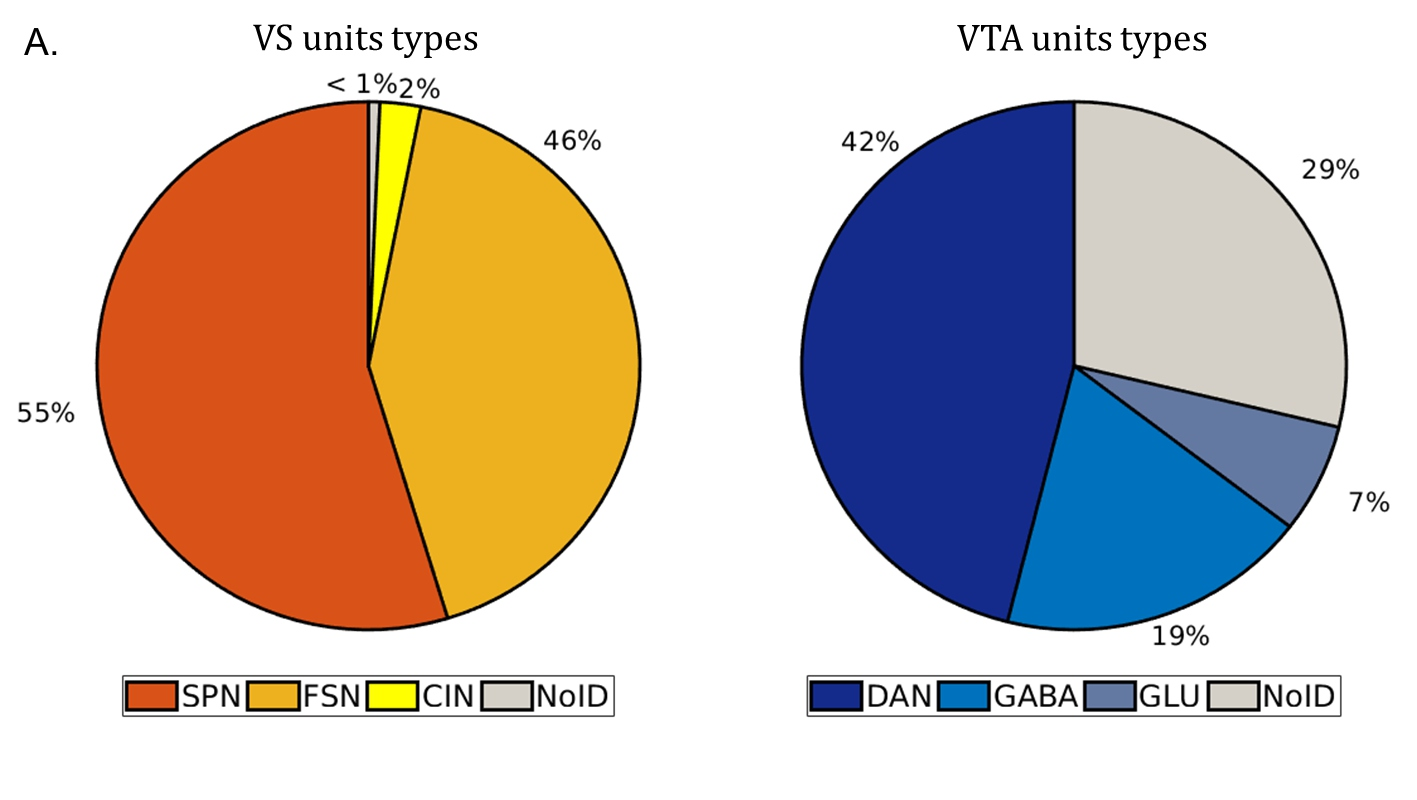
\includegraphics[scale=0.35]{figures/PieRegions1.pdf}
    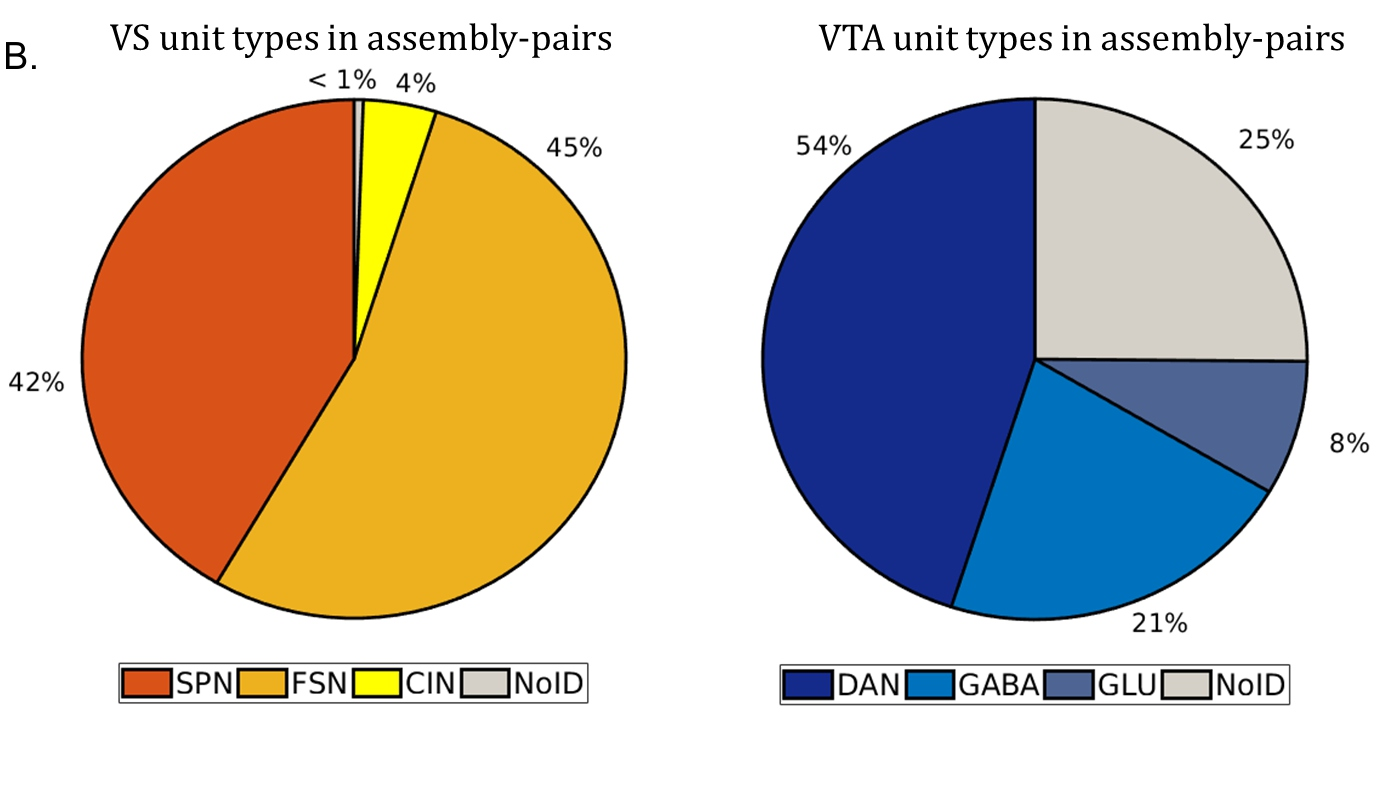
\includegraphics[scale=0.35]{figures/PieAsNotAs.pdf}
    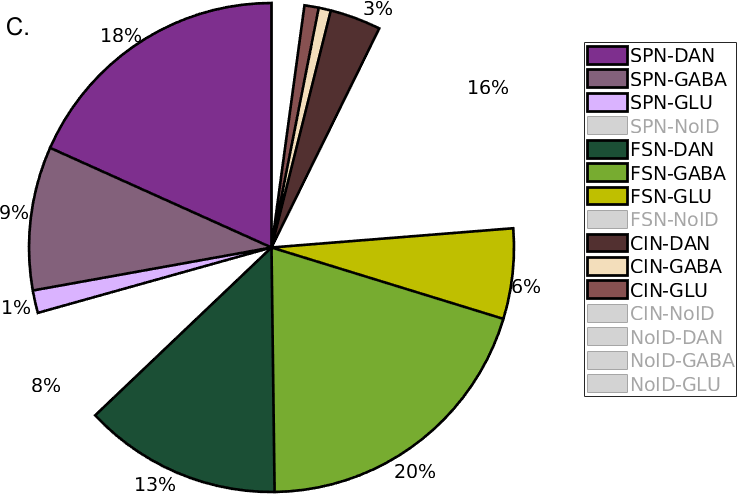
\includegraphics[scale=0.35]{figures/PieAssembliesTot1.png}
    \caption{(A.) Occurrence of classified and not classified units in VS and VTA. (B.) Occurrence of classified and not classified units of VS and VTA in inter-regional assembly-pairs. In VS, FSN occur in inter-regional pairs more often than SPN, even though more SPN than FSN were recorded.(C.) Pie charts of assemblies types. Not indicated percentage are $<1\%$. Missing pieces of cake indicates pairs that include not classified units. The four more represented inter-regional pairs, including only classified units, are pairs between fast spiking and gabaergic neurons ($20\%$), striatal projection neurons and dopaminergic neurons ($18\%$), fast spiking and dopaminergic units ($13\%$) and striatal projection and gabaergic units ($9\%$). }
    \label{fig:PieAssembliesTot}
\end{figure}
We hypothesize that the formation of inter-regional asemblies  depended on the cell-types; to verify this hypothesis we conducted for each of the two regions a Pearson's $\chi^2$ test. Of the classified unit types, only the ones detected at sufficient frequencies could tested for reasons of statistical power: namely putative striatal projection neurons (pSPN) and fast spiking neurons (FSN) in VS, and dopaminergic and gabaergic units in VTA. Only few striatal cholinergic interneurons and VTA glutamatergic units were detected are poorly represented in the examined data-set, and in the entire work and therefore not amenable to statistical analysis. We therefore focused on the four most prominent neuron types and the cell assembly pairs formed between those units.\\Whether the recorded unit may or may not be part of an inter-regional pair is described  in the contingencies tables \ref{tab:chi2_asnotasVS}, \ref{tab:chi2_asnotasVTA}. In the contingencies tables, the number (compared to the expected values indicated in parentheses) of specific cell types in inter-regional pairs were reported with $\chi^2$ statistic p-values. For each test the $\alpha$ significance level was fixed at $0.05$, unless otherwise specified.
\begin{table}[H]
    %\centering
\begin{tabular}{ |p{3cm}|p{3cm}|p{3cm}| }
 \hline
 \multicolumn{3}{|c|}{Pearson$'$s $\chi^2$ test VS unit type and inter-regional pair relationship} \\
 \hline
 & In pairs & Not in pairs\\
 \hline
 SPN & 153 (197.64) & 253 (208.36) \\
 \hline
 FSN & \textbf{197 (156.36)} & 116 (164.64)\\
 \hline
 \multicolumn{3}{|c|}{$\chi^2$ statistic  45.13}\\
 \multicolumn{3}{|c|}{p-value = $1.8\times10^{-11}$}\\
 \hline
 \multicolumn{3}{|c|}{$\chi^2$ statistic Yates correction 44.12}\\
 \multicolumn{3}{|c|}{p-value = $3.1\times10^{-11}$}\\
 \hline
\end{tabular}
\caption{Pearson's $\chi^2$ contingency table with $\chi^2$ value and p-value. Unit-types and inter-regional pairs formation are correlated in Ventral Striatum.}
\label{tab:chi2_asnotasVS}
\end{table}
\begin{table}[H]
    %\centering
\begin{tabular}{ |p{3cm}|p{3cm}|p{3cm}| }
 \hline
 \multicolumn{3}{|c|}{Pearson's $\chi^2$ test VTA unit-type and inter-regional pair relationship} \\
 \hline
 & In pairs & Not in pairs\\
 \hline
 DAN & 86 (90.604) & 31 (26.40) \\
 \hline
 GABA & 41 (36.40) & 6 (10.60)\\
 \hline
 \multicolumn{3}{|c|}{$\chi^2$ statistic  3.62}\\
 \multicolumn{3}{|c|}{p-value = 0.057}\\
 \hline
\end{tabular}
\caption{Pearson's $\chi^2$ contingency table with $\chi^2$ value and p-value. Unit-types and inter-regional pairs formation are not correlated in Ventral Tegmental Area.}
\label{tab:chi2_asnotasVTA}
\end{table}
A relationship between unit types and inter-regional pairs formation was found only in VS. In VS the $\chi^2$ statistic value is 45.13 (44.12 using Yates correction), that gives a p-value of $1.8\times10^{-11}$ ($3.1\times10^{-11}$).{\color{red}{The result confirms our hypothesis that neuron-type in VS effects the formation of inter-regional assembly-pairs. Rephase!!!!!!!}}\\A similar test was conducted in VTA, with a resulting $\chi^2$ statistic of $3.62$ and a p-value of $0.057$, not significant at $\alpha = 0.05$ level. We therefore conclude that in VTA different neuron-types had more equal probabilities to form inter-regional pairs.\\
 We have shown above how often VS and VTA units occur in assemblies. We next analyzed if specific inter regional pair-types occur systematically more often than others. The occurrence of assembly-types for the recorded units is shown in the pie-chart of fig.\ref{fig:PieAssembliesTot} (bottom). Not indicated percentages are $< 1\%$.  Missing pieces of cake indicates pairs that include not classified units. Selecting only classified units, four assemblies types occurred more often than other, they were pairs formed by fast spiking and gabaergic neurons (20$\%$), striatal projection neurons and dopaminergic neurons (18$\%$), fast spiking and dopaminergic units (13$\%$) and striatal projection and gabaergic units (9$\%$).\\
To see whether assembly types occur by chance and whether there is a relationship between the unit type activated in one region and the resulting assembly pairs, again a Pearson's $\chi^2$ test was conducted. Specifically, given the relative frequency of certain types of assemblies, we hypothesize a preference for fast spiking neurons with gabaergic neurons (and/or vice-versa) and a preference for striatal projection neurons with dopaminergic neurons (and/or vice-versa). The $\chi^2$ test were performed on the directional pairs ($lag\neq0$) and separately on $VS\rightarrow VTA$ ($lag>0$) and $VS\leftarrow VTA$ ($lag<0$). In both cases, the p-values of $\chi^2$ test were significant at the confidence level $\alpha = 0.05$, thus the $\chi^2$ test confirmed a dependence between the cell-type and the resulting inter-regional assembly pair. In direction $VS\rightarrow VTA$ the p-value was $2\times10^{-4}$ ($p=4\times10^{-4}$ using Yates correction), in direction $VS\leftarrow VTA$: $p=9\times10^{-3}$ ($p=0.017$ using Yates correction). The contingency and the results of the $\chi^2$ tests are shown for the two directionalities in tables \ref{tab:chisquare_vsvta} and \ref{tab:chisquare_vtavs}. The activated cell types of the leading region are indicated in the rows,  the coupled selected cell types of the follower region in the columns. In the table-cells the number of pairs between the two cell-types and in brackets the expected values. Both in $VS\rightarrow VTA$ and in $VS\leftarrow VTA$ directionality the real values of couples $SPN+DAN$ and $FSN+GABA$ exceed the expected values.\\ 
\begin{table}[H]
    %\centering
\begin{tabular}{ |p{3cm}|p{3cm}|p{3cm}| }
 \hline
 \multicolumn{3}{|c|}{Pearson's $\chi^2$ test ($VS \rightarrow VTA$)} \\
 \hline
 & DAN pairs & GABA pairs\\
 \hline
 SPN & 76 (63.77) & 35 (47.23) \\
 \hline
 FSN & 32 (44.23) & 45 (32.77)\\
 \hline
 \multicolumn{3}{|c|}{$\chi^2$ statistic  13.47}\\
 \multicolumn{3}{|c|}{p-value = $2\times10^{-4}$}\\
 \hline
 \multicolumn{3}{|c|}{$\chi^2$ statistic Yates correction 12.39}\\
 \multicolumn{3}{|c|}{p-value = $4\times10^{-4}$}\\
 \hline
\end{tabular}
\caption{Pearson's $\chi^{2}$ test contingency table. We test the dependency between the neuron type in VS and the neuron type in VTA with which the pair is formed, for pairs with specific directionality $VS \rightarrow VTA$. The $\chi^2$ test show a dependency among variables, meaning that resulting pair depends on the neuron types involved.}
\label{tab:chisquare_vsvta}
\end{table}

\begin{table}[H]
\begin{tabular}{ |p{3cm}|p{3cm}|p{3cm}| }
 \hline
 \multicolumn{3}{|c|}{Pearson$'$s $\chi^2$ test ($VS \leftarrow VTA$)} \\
 \hline
 & SPN pairs & FSN pairs\\
 \hline
 DAN & 18 (12.06) & 29 (34.94) \\
 \hline
 GABA & 11 (16.94) & 55 (49.06)\\
 \hline
 \multicolumn{3}{|c|}{$\chi^2$ statistic  6.73}\\
 \multicolumn{3}{|c|}{p-value = 0.009}\\
 \hline
 \multicolumn{3}{|c|}{$\chi^2$ statistic Yates correction 5.65}\\
 \multicolumn{3}{|c|}{p-value = 0.017}\\
 \hline
\end{tabular}
\caption{Pearson$'$s $\chi^{2}$ test contingency table. We test the dependency between the neuron type in VTA and the neuron type in VS with which the pair is formed, for pairs with specific directionality $VS \leftarrow VTA$. The $\chi^2$ test show a dependency among variables, meaning that resulting pair depends on the neuron types involved.}
\label{tab:chisquare_vtavs}
\end{table}
\section{Cross-/intra- area interactions time scales}
\label{sec:TimeScales}
In the previous session we have seen that in Ventral Striatum the neuronal occurrence in assembly depends on the cell-types, and specifically pallidal units (FSN) occur more in assembly than striatal projection units. Furthermore we have seen that, in directional assembly, the combination among cell types is non-random, rather cell types prefer specific cell types to form inter-regional pairs.
With these analysis we exhaustively described the cell types occurrence in Ventral Striatum-Ventral Tegmental Area interactions.\\Time scales involved in the cross-area interactions remained to be examined and are argument of this chapter, together with a comparison with intra-area interaction time scales.\\
Detecting assemblies at any time scale, the detection algorithm dissect the time scales involved in pairs-interactions. A set of bin widths $\Delta \in \{\Delta_{min}...\Delta_{max}\}$ is provided as input, so that spike patterns can be detected at different bin-size, pairs are tested at all possible bin widths, then for each assembly, the width $\Delta^*$ associated with the lowest p-value may be defined as its characteristic temporal precision (see \hyperref[chap:AssemblyMethod]{Chapter~ \ref*{chap:AssemblyMethod}}).
In figure \ref{fig:BinDistr} is shown the temporal scale ($\Delta$) distribution of VS-VTA pair-interactions.
In figures \ref{fig:BinDistrVS} and \ref{fig:BinDistrVS} are shown VS-VS and VTA-VTA time-scale interactions distribution respectively.\\
\begin{figure}[H]
%\centering
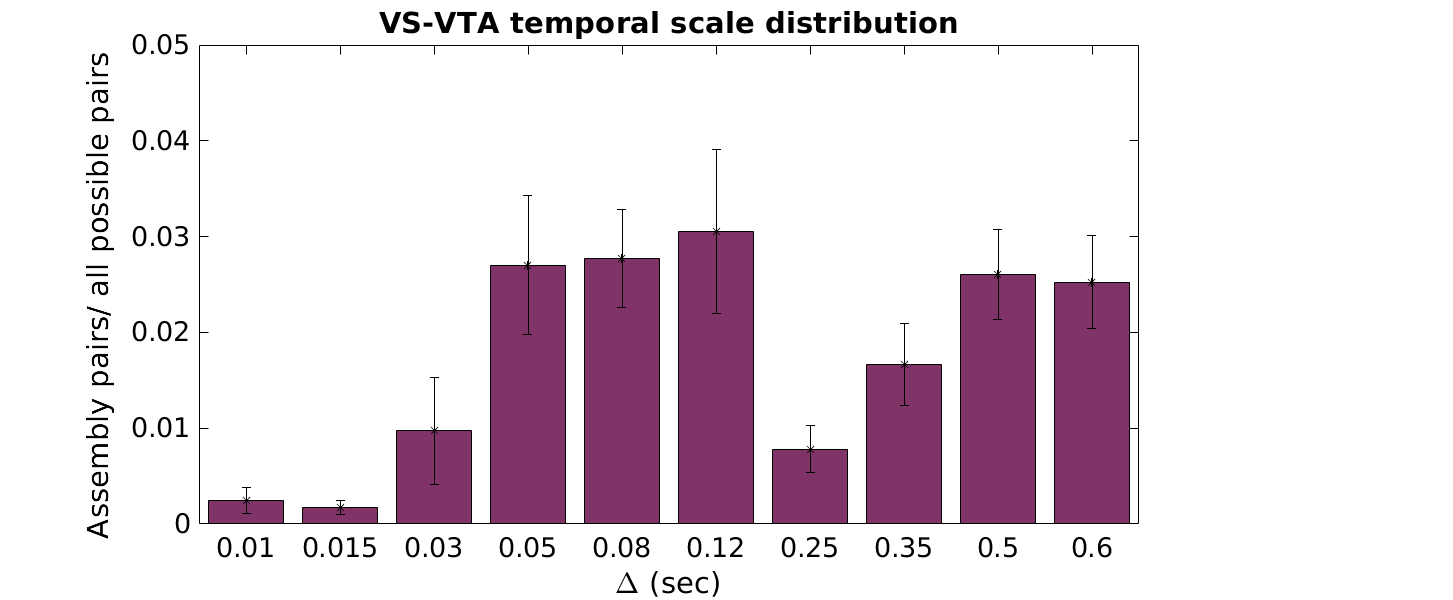
\includegraphics[scale=0.5]{figures/VS_VTA_Short1.png}
\caption{Bin distribution for inter-regional pairs. VS-VTA pairs show a bimodal distribution, revealing two temporal scale involved in inter-regional activation patterns.}
\label{fig:BinDistr}
\end{figure}
\begin{figure}[H]
%\centering
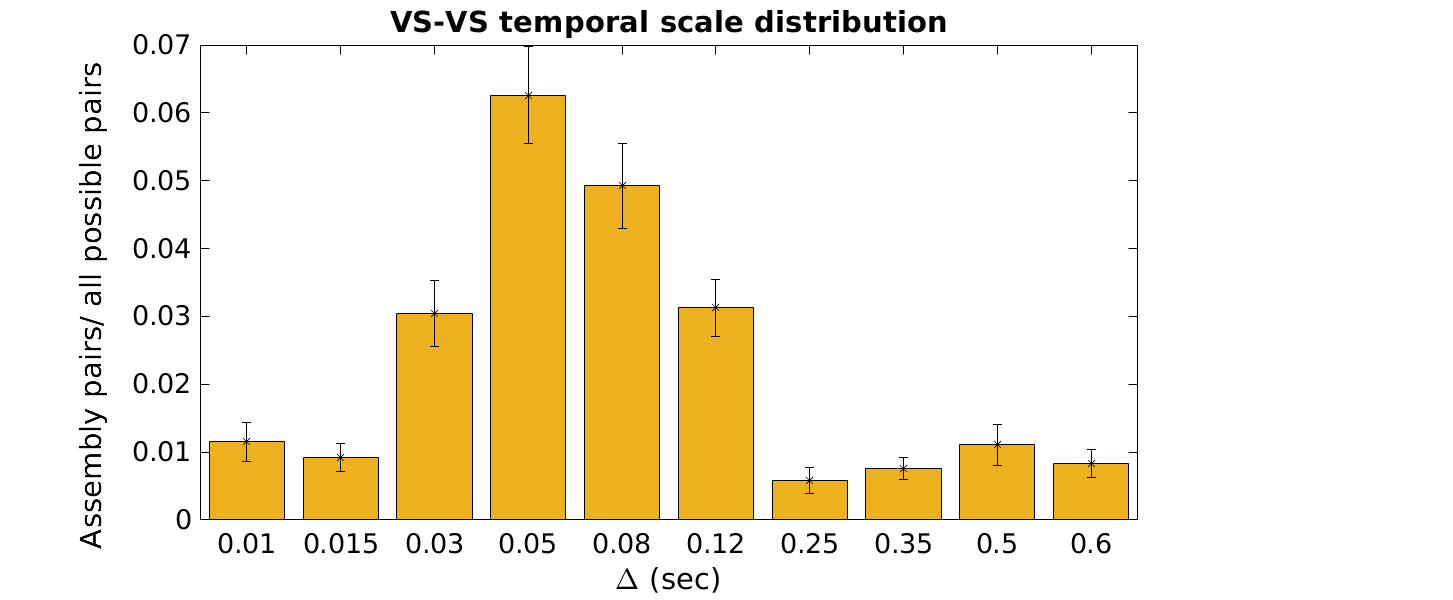
\includegraphics[scale=0.5]{figures/VS_VS_S.png}
\caption{VS-VS pairs are more precise than VS-VTA pairs and the bin distribution presents a peak at 50 $ms$}
\label{fig:BinDistrVS}
\end{figure}
\begin{figure}[H]
%\centering
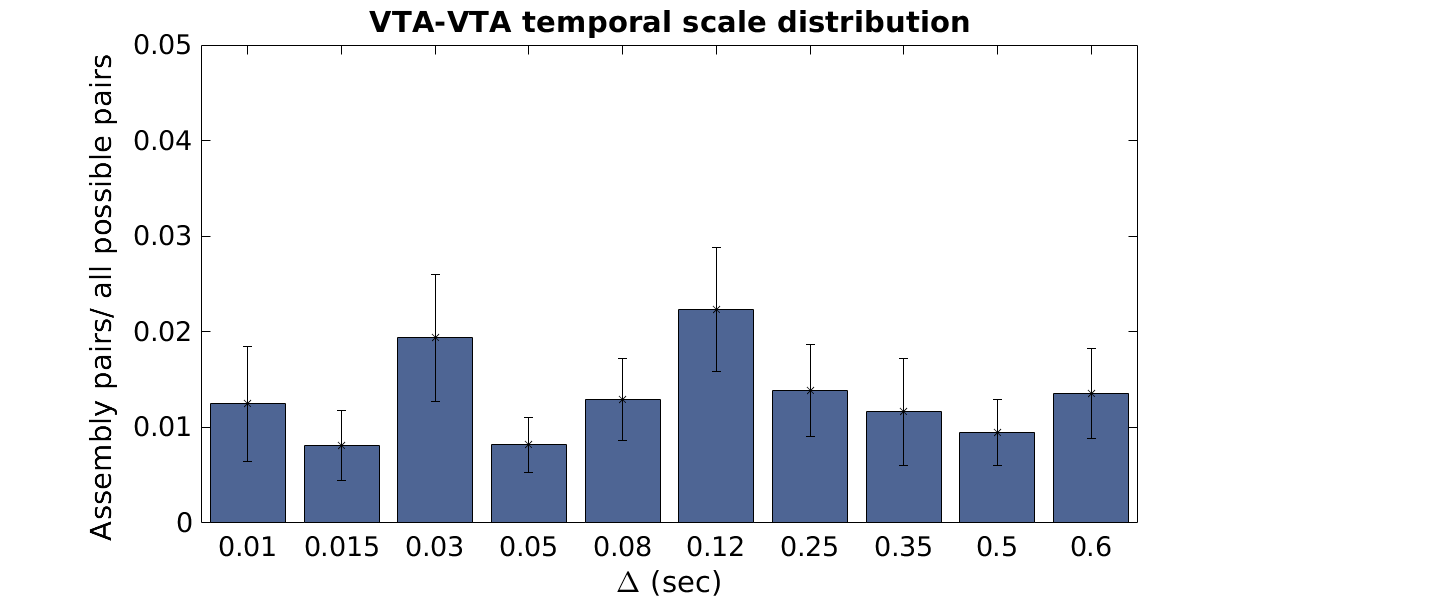
\includegraphics[scale=0.5]{figures/VTA_VTA_S.png}
\caption{VTA-VTA temporal scale distribution does not present any peak.}
\label{fig:BinDistrVTA}
\end{figure}
A comparison among inter-regional pairs (VS-VTA pairs) and intra-regional pairs (VS-VS pairs and VTA-VTA pairs) show interesting differences, that we are going to analyse.\\
While we observed assemblies of temporal precision at the scale of few tens of milliseconds only within either VS or VTA, assemblies of lower temporal precision were detected across VS-VTA units. Inter-regional VS-VTA interactions have a bimodal time-scales distribution with peaks around 80 $ms$ and one 1.6 $sec$, revealing two time scales involved in VS-VTA interaction, the first, more precise, ranged from 10 $ms$ to 250 $ms$, and the second including broader bin sizes; from which we consequently argue a complex interaction circuit effect, reflecting in inter-regional pairs.\\Bimodality is a characteristic specific of VS-VTA interactions, not present in VTA-VTA, or VS-VS interactions: intra-regional VTA-VTA pairs do not present any peak in time scales distribution, whereas intra-regional VS-VS bin size distribution is peaked around 50 $ms$.  
\subsection{SPN-FSN time scales interactions *}
\label{sec:SPN-FSN_Bin}
Fast spiking neurons population has broad firing rate, and according to the firing rate, sub-populations of the neurons classified as fast spiking neurons in first place can show different characteristic in terms of time-scales and length of interactions, or/and feature coding ({\color{red}ask for paper to cite}).\\From the distribution of mean firing rate of the recorded FSN was possible to define two sub-populations, those last do not present different characteristic when their units are coupled in assembly with a VTA neuron, however it worth to mention them in relation to their time-scales interactions with SPN. We report in figure \ref{fig:FSNsFireHisto} the histogram of FSNs mean firing rate, from which is possible to distinguish two sub-populations, that we will call FSNs low and FSNs high: the first characterized to have mean firing rate below $45 Hz$ and the latter has mean firing rate equal or above $45 Hz$.\\
\begin{figure}
    \centering
    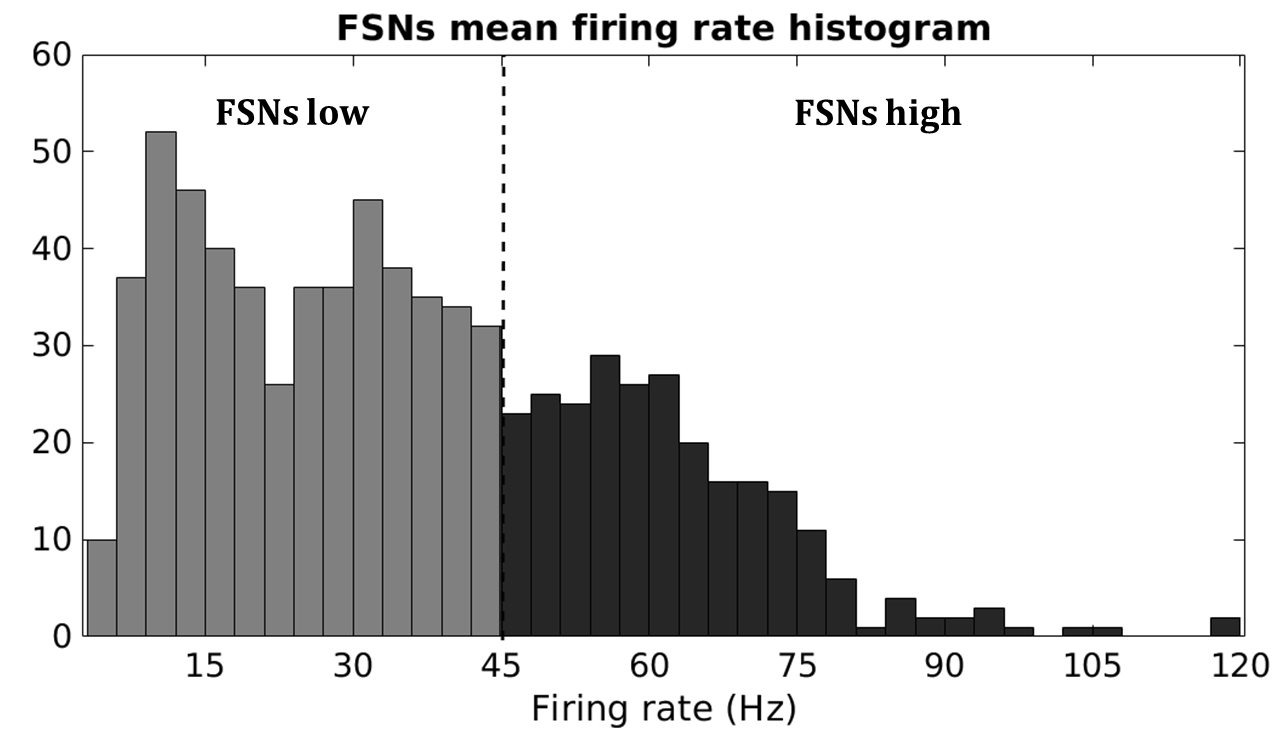
\includegraphics[scale=0.6]{figures/FSNFiringRateLightDark.pdf}
    \caption{Histogram of FSNs mean firing rate. We can distinguish two populations of FSNs: FSN low-firing-rate population (FSN-low), that are light grey in the graph, characterized by having a firing rate below 45 $Hz$, and FSN high-firing-rate population (FSN-high), in dark grey, characterized by having a firing rate from 45 $Hz$ upwards.}
    \label{fig:FSNsFireHisto}
\end{figure}
\begin{figure}
    \centering
    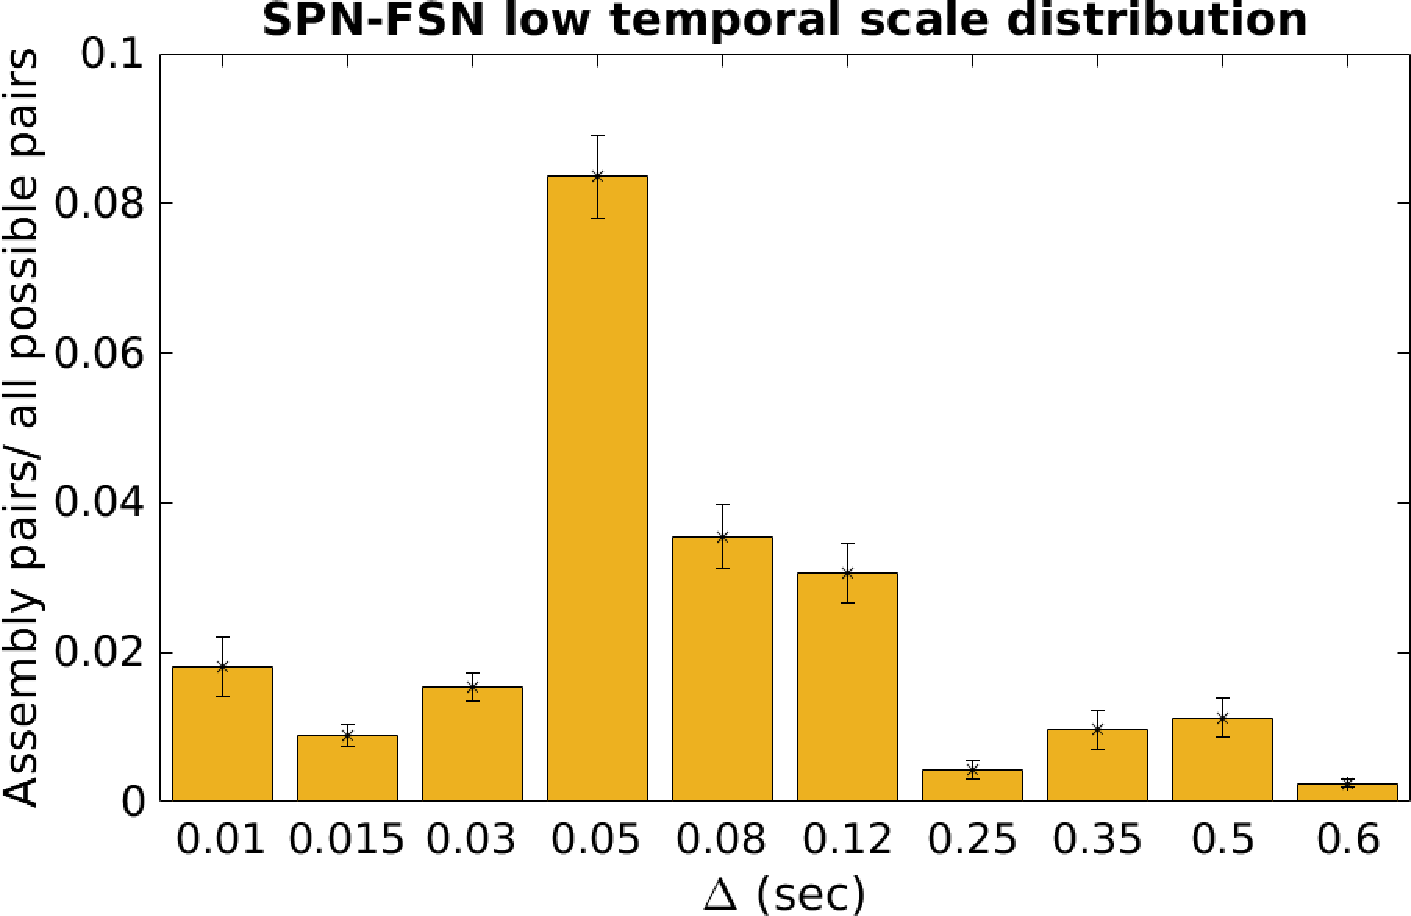
\includegraphics[scale=0.5]{figures/SPN_FSNlow1.pdf}
    \caption{SPN-FSN-low temporal scale distribution is peaked at 50 $ms$. A good portion of SPN-FSN-low pairs is detected also at 80 $ms$ and 120 $ms$.}
    \label{fig:SPN_FSNlowBin}
\end{figure}
\begin{figure}
    \centering
    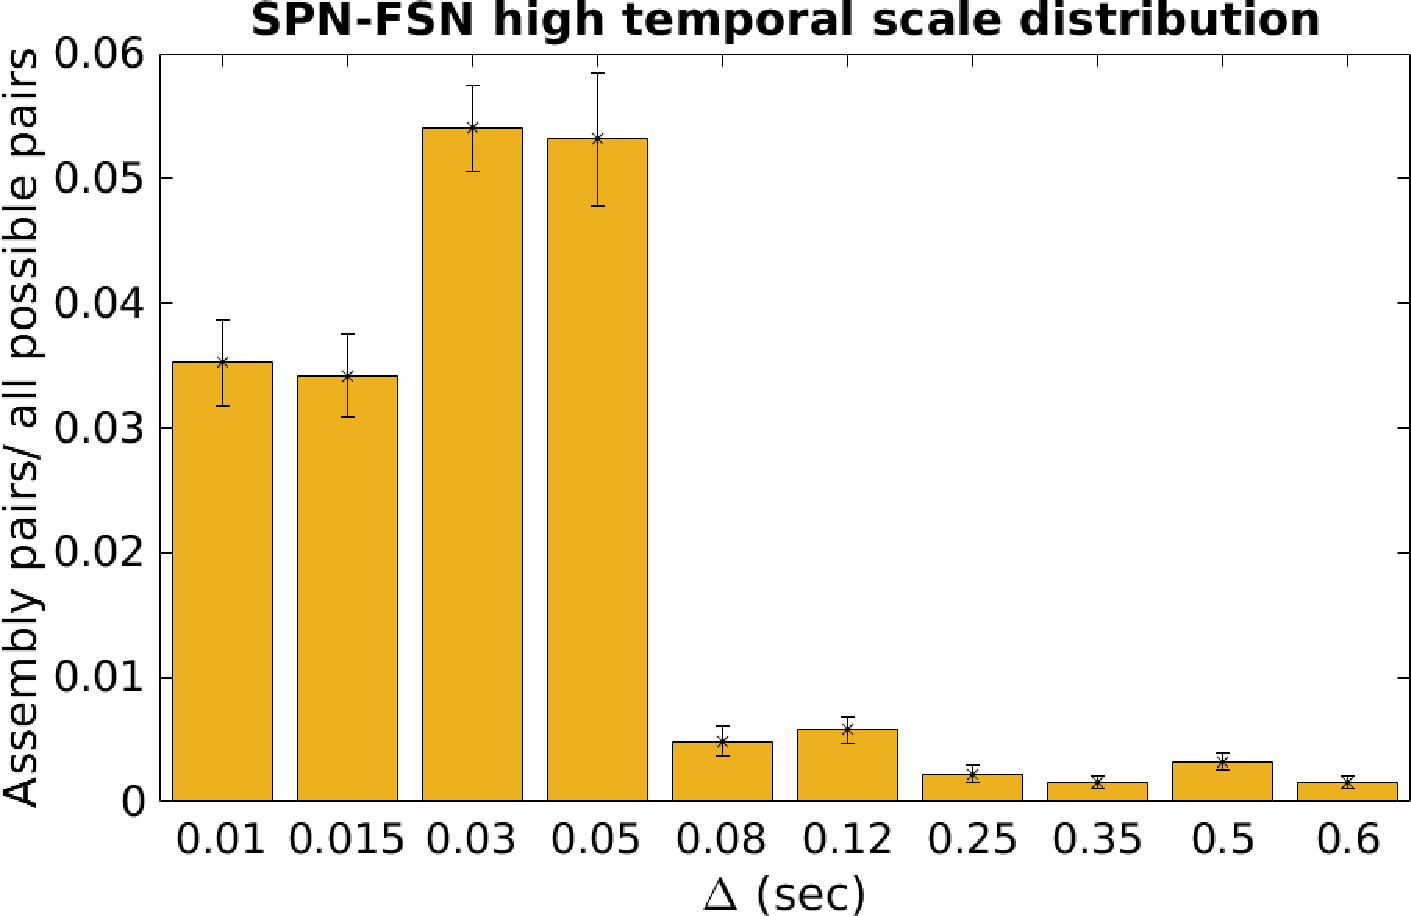
\includegraphics[scale=0.5]{figures/SPN_FSNhigh1.pdf}
    \caption{SPN-FSN-high pairs are almost exclusively detected at very precise time scales, namely from 10 $ms$ to 50 $ms$.}
    \label{fig:SPN_FSNhighBin}
\end{figure}
In VS we noticed differences between SPN-FSN-low pairs and SPN-FSN-high bin size distributions. SPN-FSN-low bin distribution pair is peaked at 50 $ms$, and another good portion of those pairs is detected at the two next bin sizes after the peak, 80 $ms$ and 120 $ms$ (fig. \ref{fig:SPN_FSNlowBin}); whereas SPN-FSN-high pairs are essentially only detected at more precise temporal scale (fig.\ref{fig:SPN_FSNhighBin}).\\We conclude that those two pair-types give a specific contribution to the global VS-VS temporal scale distribution. The variety of time scales involved in intra- or cross- area interactions in the studied regions emphasizes the complexity of the interaction circuit.
\section{Directionality} 
\label{sec:Directionality}
We had found in \hyperref[sec:TimeScales]{Section~\ref*{sec:TimeScales}} that inter-regional interactions have two characteristic time scales, which led us to consider more precise ($\Delta \in [0.01,0.25] ms$) and broader ($\Delta \in [0.25,0.6] ms$) VS-VTA pairs separately in the further study of directionality.\\We recall that one of the output of the cell-assembly algorithm is the inter-units activation lag of the assembly and, when we restrict the investigation to inter-regional pairs, the lag value tells us the distance in activation between the two region while the sign of the lag indicates the direction of the activation, namely which region became activated first and which one follows.\\
In fig.\ref{fig:LagInSecAll} we show the lag distribution for detected inter-regional pairs in the two characteristic time scales of interaction. As indicated in the plot, a positive lag means VS is functionally leading the VTA activation and a negative lag indicates the opposite direction.\\Interestingly lag distributions of precise and broad pairs are asymmetric, indicating that preferentially the VS activation leads the activation of the VTA. The two lag distributions show however remarkable differences: the lag distribution of broader pairs is fat-long tailed, because a good portion of pairs detected with long activation lag ($lag > 1 sec$), whereas preciser pairs lag distribution has thin tails: almost all pairs detected in precise time scale have short lag ($|lag| < 1 sec$), and a good portion of pairs is detected within a lag value of 0.5 $sec$.\\
We focused the study on the more precise temporal scale, in such a way that temporal scale interactions were separated to typical task-related time scales, as e.g. the length of the odor duration, which cover typically an interval from 1.0 $sec$ to 1.5 $sec$.\\
We observed that the directional assemblies are composed of striatal projection neurons leading dopaminergic neurons (SPN-DAN pairs), all the other pair-types do not show a clear preferred directionality. Furthermore, inter-unit activation lags of assemblies containing pallidal neurons (FSN) are shorter than those containing striatal projection neurons (SPN), compatibly with assumed connectivity. In fig.\ref{fig:LagInSec4typo} is shown the lag distribution for the four principal pair-types.\\
VTA dopaminergic neurons were laser tagged in first place, we can use the laser tagged units as control to validate the dopaminergic neurons classification; in fig.\ref{fig:LagInSecLaser} is shown the lag distribution of laser tagged dopaminergic units coupled with SPN and FSN. Is clear the similarity between the lag distribution of pairs containing laser tagged dopaminergic units and the lag distribution of the pairs containing classified dopaminergic units, in fact SPN-laser DAN pairs show directionality in direction $VS\rightarrow VTA$, whereas FSN-laser DAN are not directional, as we expected from the results obtained using classified units, which confirms the validity of the adopted classification.\\
\begin{figure}[H]
\centering
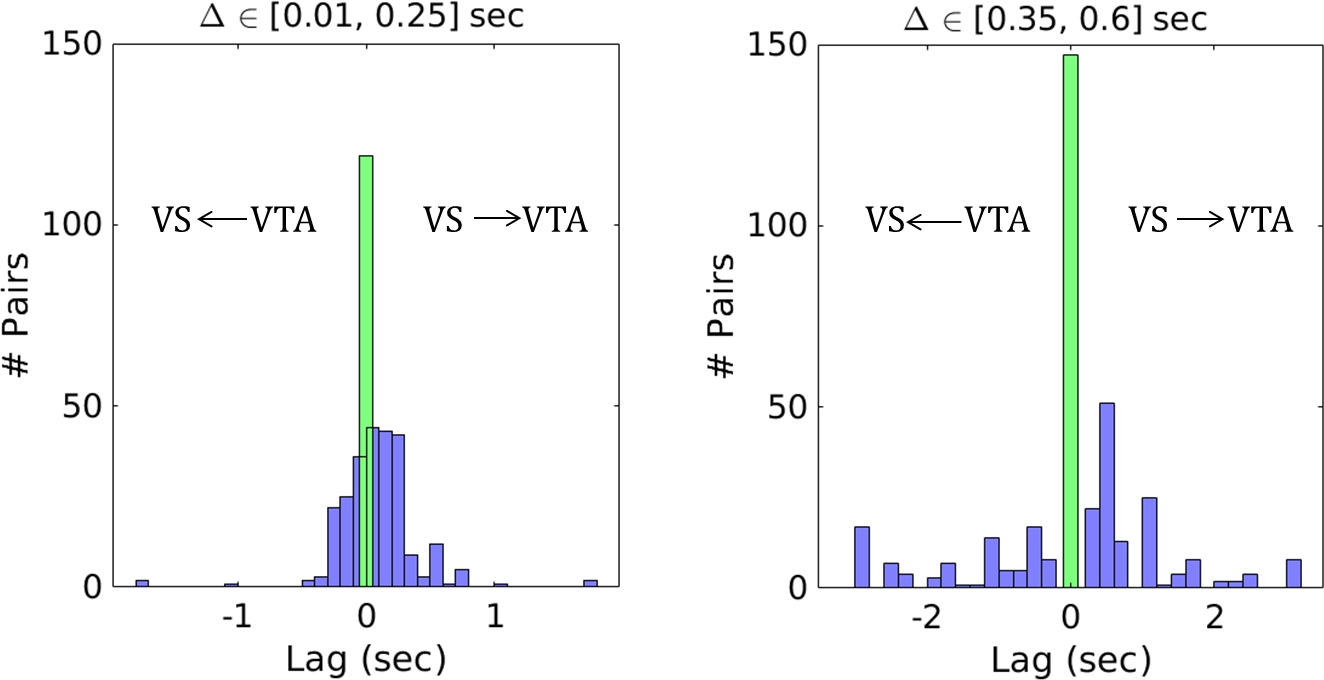
\includegraphics[scale=0.6]{figures/LagGeneral1.pdf}
\caption{Lag distribution for VS-VTA pairs in seconds. In green the synchronous pairs. On the left, lag distribution for pairs detected in more precise time scale. Slight distribution asymmetry indicates directionality in the direction of $lag > 0$, meaning a predominance of pairs in which VS leads VTA. On the right, the lag distribution for pairs detected in the broader time scale, it presented as an asymmetric fat-tailed distribution.}
\label{fig:LagInSecAll}
\end{figure}
\begin{figure}[H]
\centering
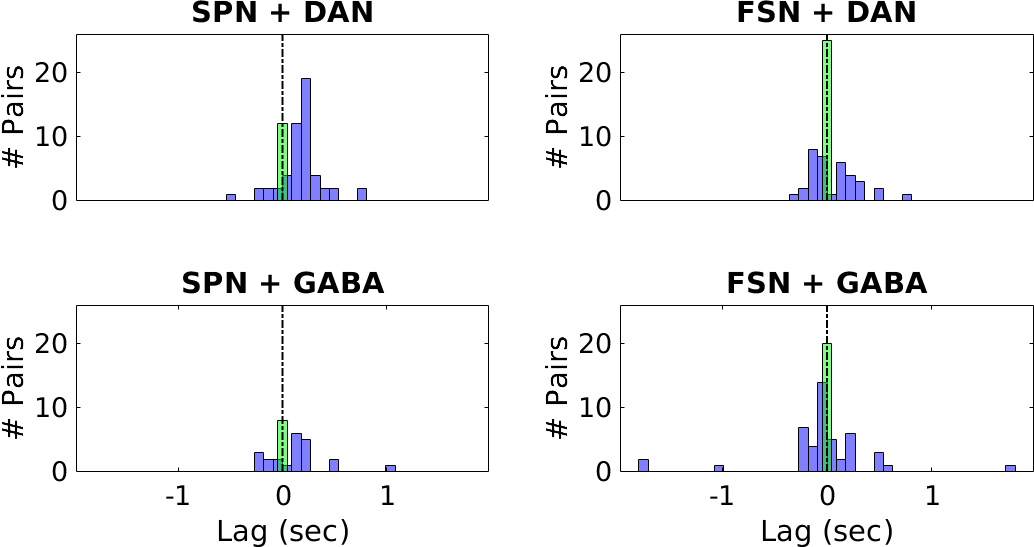
\includegraphics[scale=0.5]{figures/LagSec4Typo3VS.png}
\caption{Lag distribution of four more represented pair-types in precise time scale. Only SPN-DAN pairs show a preferred directionality, namely $VS\rightarrow VTA$.}
\label{fig:LagInSec4typo}
\end{figure}
\begin{figure}[H]
\centering
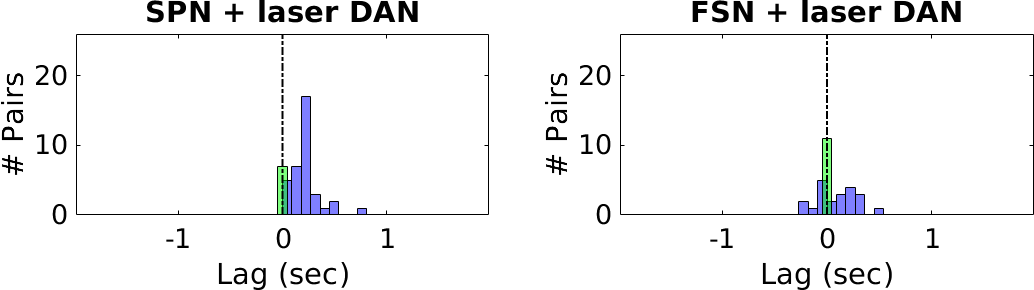
\includegraphics[scale=0.5]{figures/LagSecLaser3VS.png}
%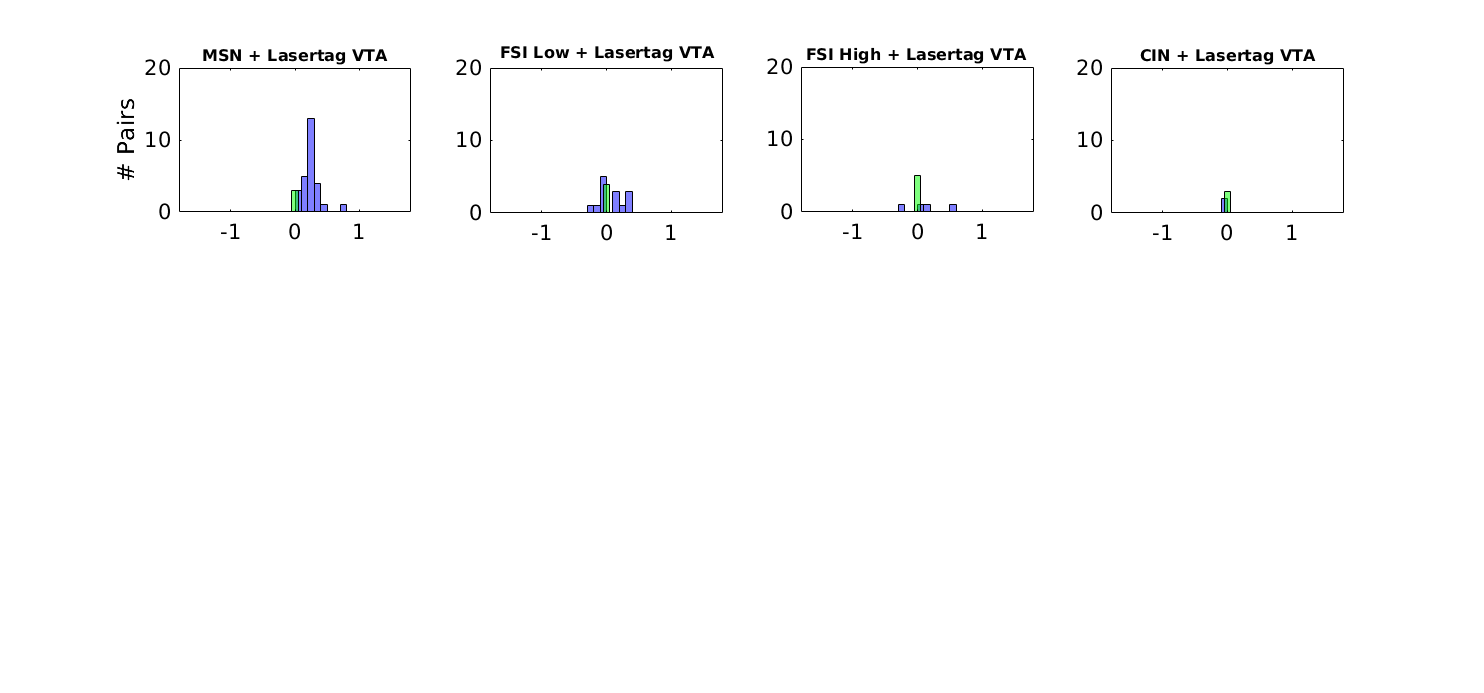
\includegraphics[scale=0.4]{figures/OnlyLaserOriz.png}
\caption{Lag distribution of laser tagged dopaminergic units in pair with SPN and FSN units, in precise time scale. Lag distributions are similar to the lag distributions of classified DAN in pair with SPN and FSN, confirming the directionality expressed by SPN-DAN pairs and the validity of the classification adopted in VTA.}
\label{fig:LagInSecLaser}
\end{figure}
The kind of activation exhibited by a directional pair is exemplified for an inter-regional directional pair in fig.\ref{fig:directional_assembly}. The pair in example was detected with a bin width of $\Delta = 0.12$, and the inter-units activation lag was positive with value 0.36 $sec$. On top is shown the mean across trials of the pair activity for rewarded (grey line) and unrewarded odor (purple line) in the original phase. From the activation profile and the separation between the two activation lines one can see that the illustrated pair specifically code for rewarded odor. On bottom are shown raster plot and mean firing rate of units in assembly. x-axis origin corresponds to the odour onset, while the red line marks the end of the stimulus duration.
Looking at the activity of two neurons, the directionality exemplified by the pair is evident, in fact first the VS unit becomes active and, after a temporal delay, the activation of VTA unit follows. Raster plots show the stability of the activity across trials.\\ 
\begin{figure}
    \centering
    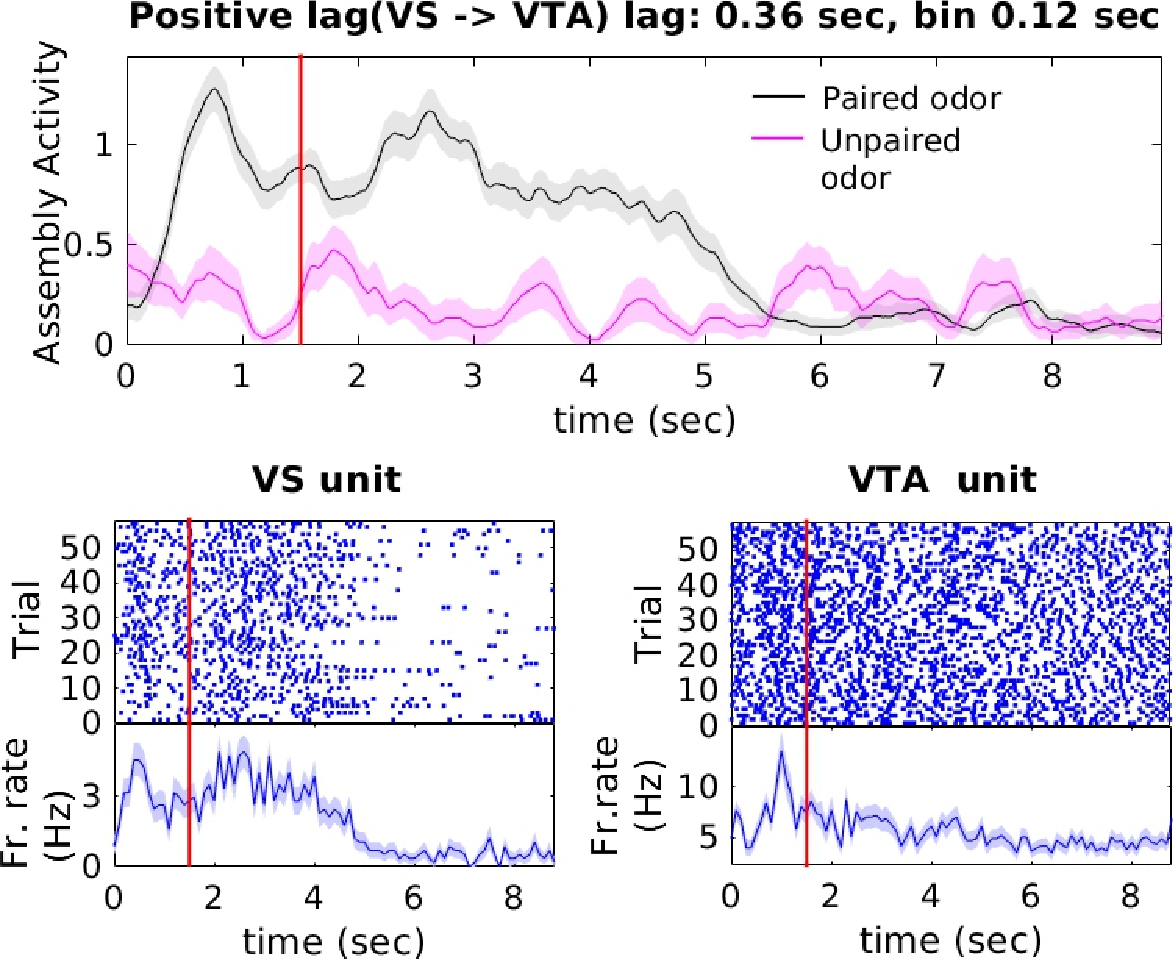
\includegraphics[scale=0.6]{figures/DirectionalAsEx1.pdf}
    \caption{Directional assembly. On top mean across trails and standard error of the activity of the pair for rewarded (grey) and unrewarded odour (purple) in the original phase. On bottom raster plot and firing rate (mean and standard deviation) of units in assembly. x-axis origin corresponds to the odor onset, while the red line marks the end of the stimulus duration. The examined assembly has a positive lag, that means VS preceding in activity VTA, from neuronal activity we can see in fact the VS unit activate before than the VTA unit.}
    \label{fig:directional_assembly}
\end{figure}
At population level time scale and directionality segregation reveals different assembly-activation patterns. In fig.\ref{fig:AsActBinLag} an example of dissection of activation patterns is shown through the heat map of inter-regional pairs activity averaged across trials in one of the paradigms of the experiment.\\Pairs exhibiting directionality $VS \rightarrow VTA$ and detected in the precise time scale ($\Delta \le 0.25$) became activated early during the odour presentation.\\The early activation at the stimulus presentation is the type of activation we expect when the animal predicts the reward, as discussed in \hyperref[sec:StateArt]{Section~\ref*{sec:StateArt}} (see fig.\ref{fig:RewPred}), moreover we have shown in fig.\ref{fig:LagInSec4typo} as the SPN-DAN pairs are directional, thus we speculate that SPN-DAN are good candidate for reward prediction (RP) coding; the investigation of this hypothesis will be argument of the next chapters.\\
\begin{figure}[h!]
    \centering
    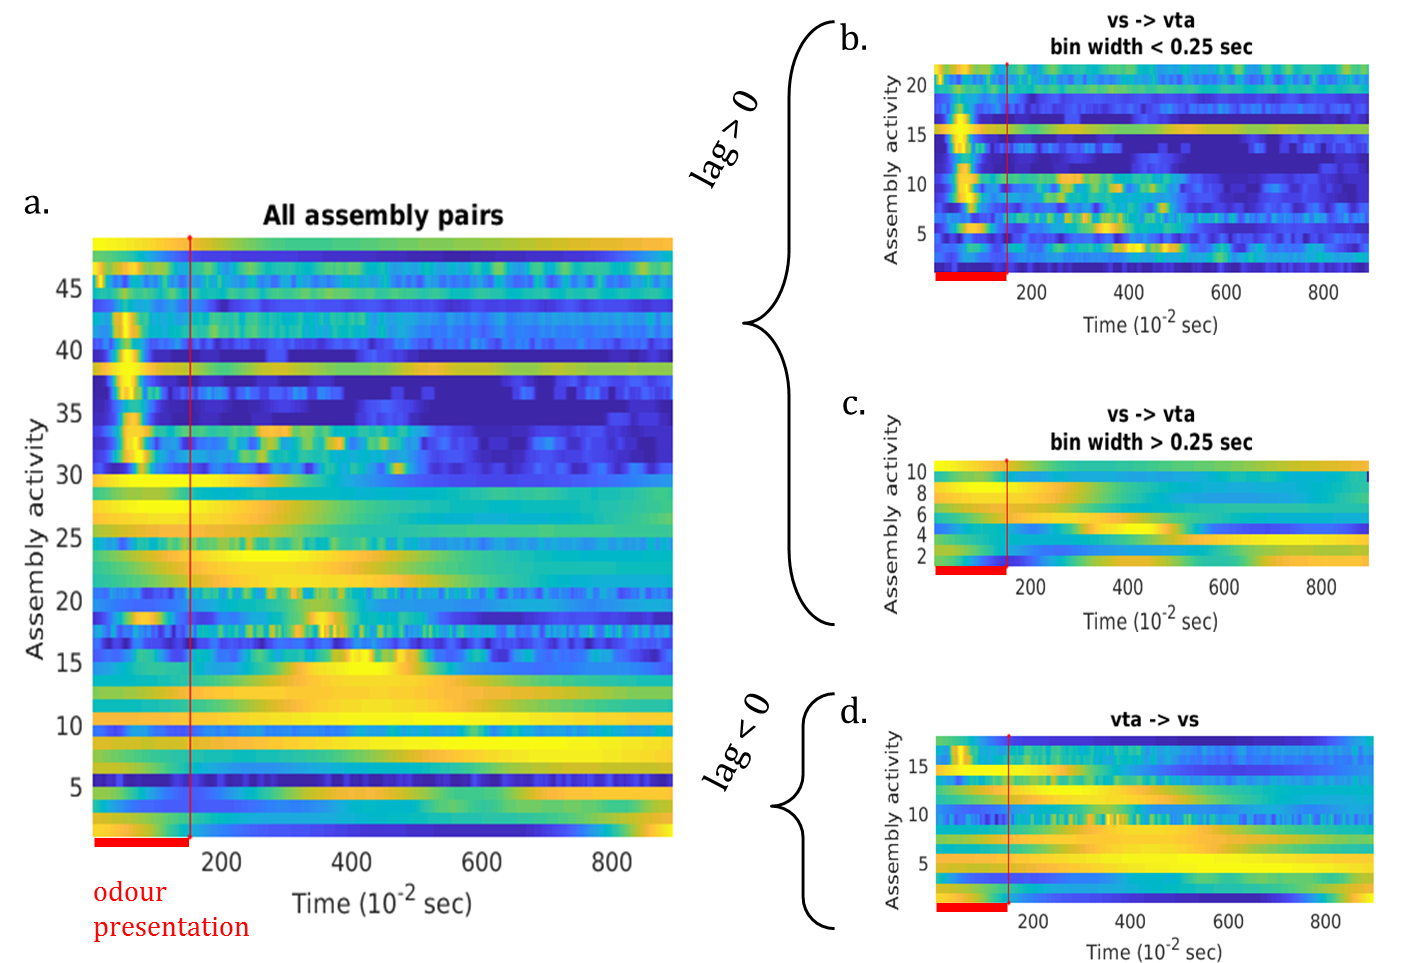
\includegraphics[scale=0.6]{figures/AsActPerBinLag1.png}
    \caption{Assembly-activation patterns given time bins and lags. In a.) heat map of inter-regional pairs in one the experimental paradigms, b,c,d. pairs of a. selected for bin size ($\Delta$) and lag: $\Delta < 0.25 s$ and $lag > 0$ (b.), $\Delta > 0.25 s$ and $lag > 0$ (c.), $lag < 0$ (d.)}
    \label{fig:AsActBinLag}
\end{figure}
\begin{figure}[h!]
    \centering
    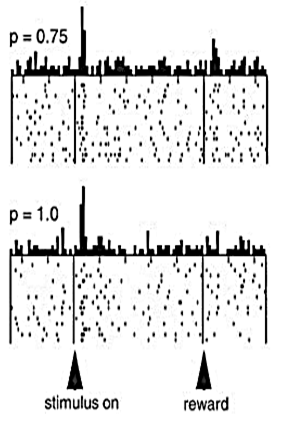
\includegraphics{figures/RewPred1.png}
    \caption{Predictive reward signal in dopamine neurons. Adapted from \cite{Fiorillo}}
    \label{fig:RewPred}
\end{figure}
\pagebreak
\section{Conclusion}
From the inter-regional time scales distribution we deduced that VS-VTA pairs have two time scales of interaction, highlighting so the complexity of VS-VTA pair interactions and underlines the importance to choose a method capable to explore different time scales.\\The two time scales involved in VS-VTA interaction were then separated to continue the study with the lag analysis, from which emerged a preferred directionality in the verse $VS\rightarrow VTA$, and specifically in pairs containing striatal projection neurons and dopamaninergic neurons.\\Different time scales of interaction and directionalities refelect different patterns of assembly-pair activity. As preliminary investigation we have shown, in a small portion of the data-set, that pairs detected at the precise time scale and exhibiting the directionality $VS\rightarrow VTA$ show a reward related signal in agreement with the prediction error coding signal.\\Since directional assemblies are formed by striatal projection neurons and dopaminergic neurons, we hypothesize that those pairs are good candidate for prediction coding. The next chapter is aimed to understand first whether directional assembly-pairs compute prediction error and if this signal is specific of directional pairs (SPN-DAN). Comparing the activity of different assembly-pair types we ask whether different assembly-pair types specialize in different coding features. The starting point of the analysis is the pair-types task related response. A systematic analysis of this is performed in \hyperref[sec:TaskResp]{Section~\ref*{sec:TaskResp}}.

 \section{Pair-types task-related pattern}
 \label{sec:TaskResp}
 {\color{red}discussion is a draft}
In the previous section we concluded that time scale segregation and directionality might reflect specific task-related coding feature. In a data subset we have shown how different time scales and directionalities reveal different assembly-pairs activity patterns.\\We have seen as well that different assembly-pairs types have different directionality distribution. SPN-DAN assembly-pairs, in particular, exhibit a clear $VS\rightarrow VTA$ directionality.\\In this section we prove that different assembly-pairs-types have different task-related activity patterns, which express different task-related feature coding.\\
To this purpose we tested the responsiveness of each assembly-pair to the conditioned stimulus (CS $+/-$) and the unconditioned stimulus (US), through an analysis of variance performed using both a paired Friedman test and a non parametric version of repeated measure Anova test, on the trial by trial assembly-pair activity. The results of the two tests are consistent each other, we choose to present here only Friedman test results, leaving summary and comparison in\hyperref[app:FriedAnova]{~Appendix\ref*{app:FriedAnova}}. The choice of non parametric tests was made to be free from gaussianity assumption.\\Time intervals were 0.5 $sec$ long, and were chosen as it follows: CS $+/-$ interval included all time steps $t \in [0, 0.5]$ $sec$ from the odor onset, CS$+/-$cont. was the window including each time $t$ satisfying $t \in [-0.5, 0]$ $sec$ before the reward retrieval, in which the the odor was still present, US interval included times $t \in [0,0.5]$ from the reward delivery. The assembly-pair activity in the listed task relevant intervals was compared with the baseline interval including times $t \in [-0.8, -0.3]$ $sec$ before the odor onset, in which no task related activity could have interfered with the spontaneous neural activity.\\In fig.\ref{fig:Baseline} is shown the heat map of the neural activity averaged across trials before and after the odor onset, during the baseline period (interval delimited by the two back lines) no activity patterns emerge besides the spontaneous neural activity.\\
\begin{figure}
    \centering
    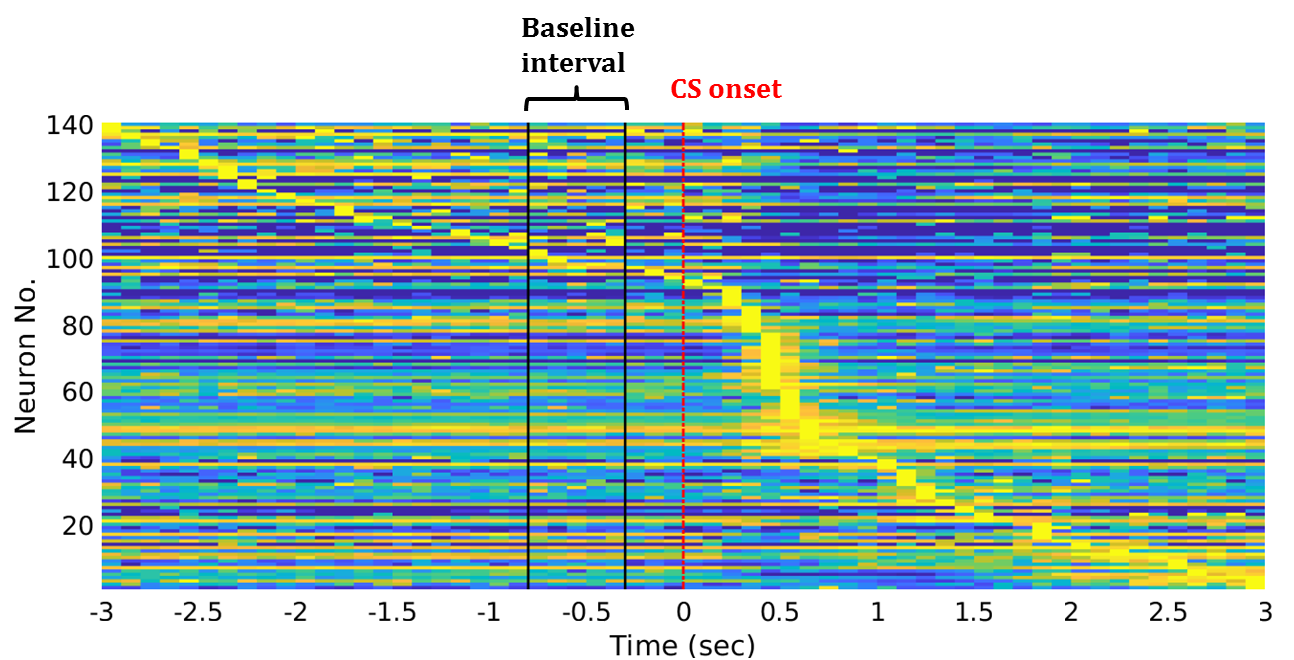
\includegraphics[scale=0.6]{figures/Baseline.png}
    \caption{Baseline interval choice. For each trial the baseline interval was a time window in which no task related activity could have interfered with the spontaneous neural activity, as shown by an example of the neural activity averaged across trials.}
    \label{fig:Baseline}
\end{figure}
Analysis of variance compares the means of several groups to test the hypothesis that they are all equal, against the general alternative that they are not all equal. This alternative was in our case too general. Hence, in the cases in which we obtained an omnibus significant $\chi^2$ test, the post-hoc procedure were designed using the matlab function $\textit{multcompare}$ whose critical values where computed with Bonferroni method.\\
In fig.\ref{fig:SPN_Ex} two examples of assembly-pairs resulting significant for Friedman test made on hit trials (correct trials when the rewarded odor was presented).\\On top a SPN-DAN pair, for which the post-hoc analysis revealed a significant difference between the baseline and the CS+ cont. groups. Interestingly we observe, in CS+ cont. window, less assembly-activity in the first trials and intense assembly-activity in the last trials, the same trend is observed in CS+ window in another pair example fig.\ref{fig:SPN_Ex}, while the opposite trend is observed for the same pair during the reward retrieval (US window).\\This dynamical responsiveness resembles a typical learning dynamic. In first trials the mouse lives an explorative period in which the rule of task has not been learnt yes, while it has been learnt at the end of the original phase. In other words in the first part of the task the animal is almost always surprised when the reward is delivered, the expectation of reward is low, while during the second part of the original phase the mouse is able to predict the reward already at the stimulus presentation, the expectation of reward increases when the rewarded stimulus is presented.\\Moreover not debated considerations in literature about Ventral Striatum and dopaminergic neurons activity related to the expectation of reward (\cite{Schultz1992} \cite{Schultz} \cite{Fiorillo}) show that in presence of probabilistic reward the response of dopaminergic units is peaked at the reward time when the probability to get the reward is low and is instead peaked at stimulus presentation when the probability to get the reward is high, VS neurons instead show a tonic response from the stimulus presentation.\\In this scenario one can says that if an assembly-pair code for reward prediction error, then the activity will be intense during the presentation of the rewarded stimulus only in the last part of the task-phase. An example of dynamic responsiveness across trials is shown in fig.\ref{fig:SPN_Ex} (top) in the CS+cont. window , and in fig.\ref{fig:SPN_Ex} (bottom) CS+ window. On the contrary at retrieval (US) we expect intense activity in first trials, related to the surprise to have the reward, and less activation in the second part of task, when the animal acquired sureness about the reward fig.\ref{fig:SPN_Ex} (bottom US window).\\
\begin{figure}
    \centering
   % 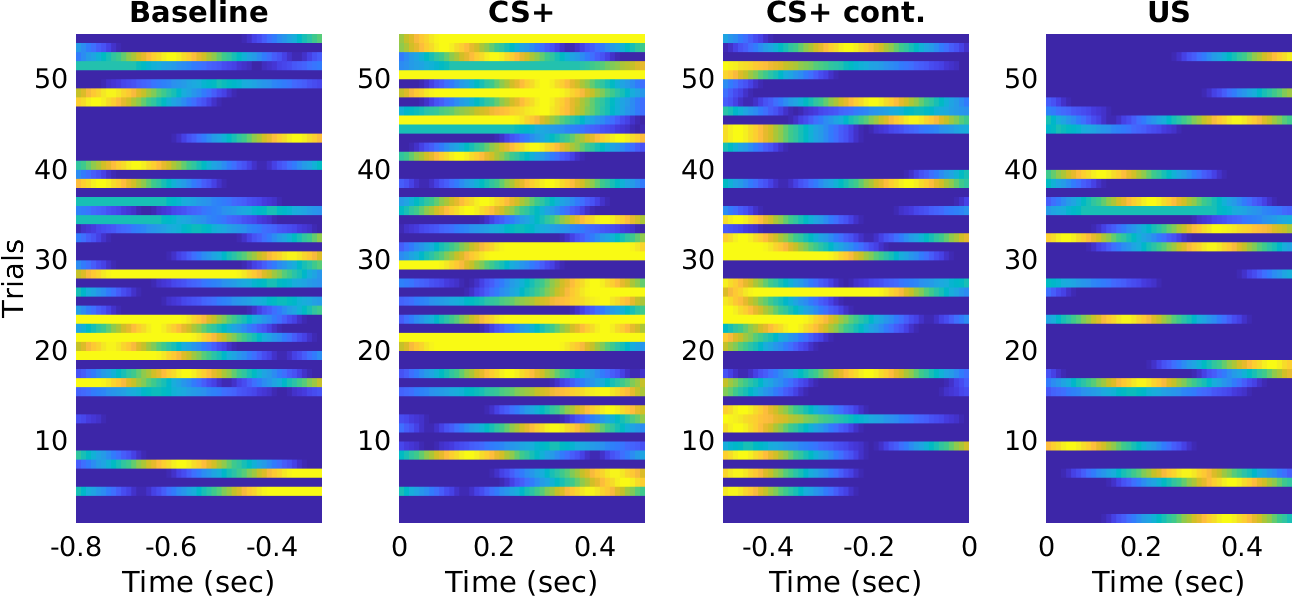
\includegraphics[scale=0.4]{figures/SPN_DANexStim1.png}
    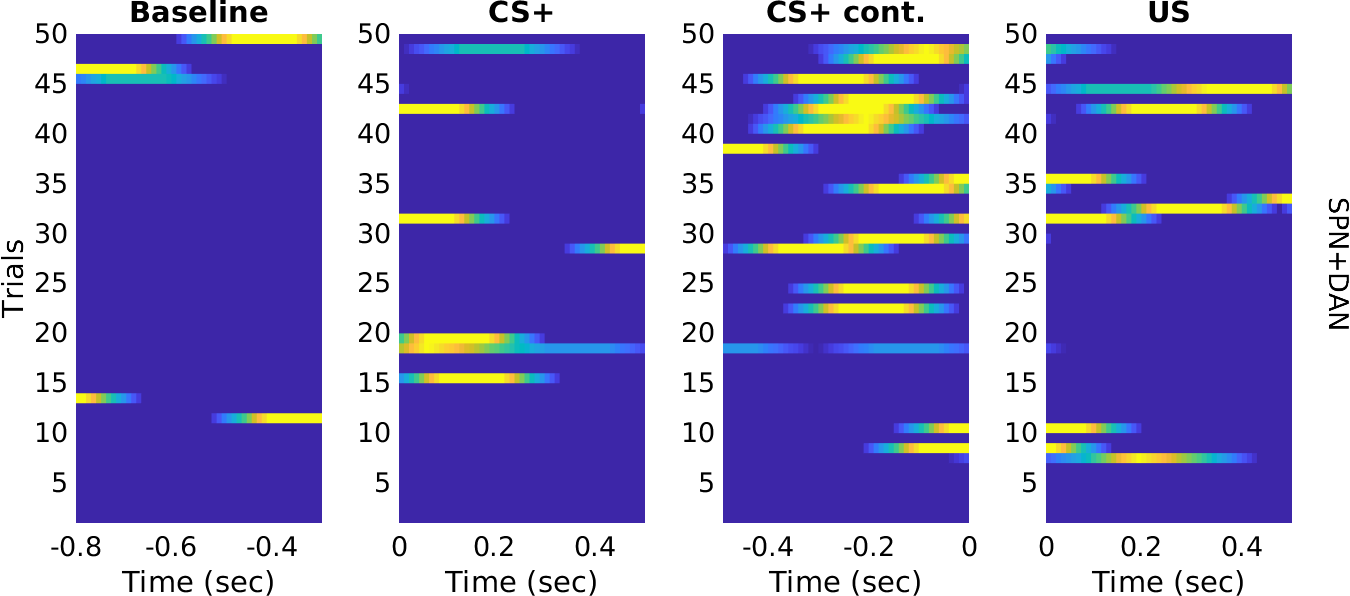
\includegraphics[scale=0.4]{figures/SPN_DANexPreRew.png}
    
   \vspace{1cm}
   
   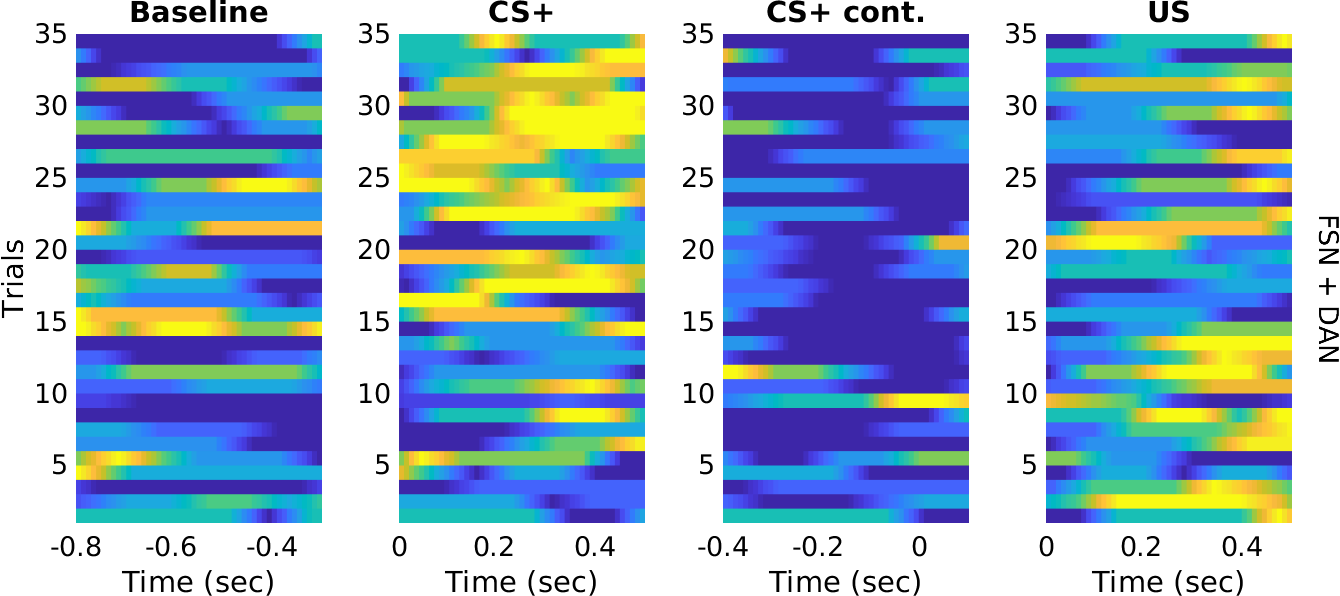
\includegraphics[scale=0.4]{figures/FSN_DANexStimRew.png}
    \caption{Example of two SPN-DAN assembly-pairs significant after the analysis of variance for which the post-hoc test shown that in both cases two groups out of for were significant different, respectively the baseline and the CS+ window (top), and the baseline and the CS+ cont. (bottom).}
    \label{fig:SPN_Ex}
\end{figure}
The two examples above show that for sure some assembly are implicated in the learning dynamic, are they all involved in prediction error computation? Do they show different coding features depending on their underlying units? To answer these questions a zoom on the reward-related response of dopamine neurons is needed.\\Despite robust evidence for dopamine units involvement in reward coding, it is hard to identify how this signal is elaborated processed by dopamine neurons. Recent works pointed out that at least two different response components are involved in reward coding and that the neuronal reward processing evolves in time from unselective sensory detection to more demanding and crucial stages of identification and valuation. The initial component, characterized by a brief activation, it occurs unselectively in response to a large variety of unpredicted events and corresponds to the large range and heterogeneous nature of potentially rewarding stimuli and object present in the environment.\\The later component defines the function of the dopamine response and reflects the evolving neuronal processing that is required to fully appreciate the value of the stimulus (\cite{Tobler2003}, \cite{Nomoto2010}, \cite{Fiorillo2013} \cite{Schultz2016}).\\
This work aims to prove this crucial point: although at single neuron level different dopamine neurons don't code specifically for one of the two components of prediction error (\cite{UchidaDop}) and they use the moment to moment reward prediction associated with environmental stimuli to compute a reward prediction error, the specificity of different components coding emerges in the assembly-pairs activity because different interactions convey different aspects of the prediction error coding.
\begin{figure}
    \centering
    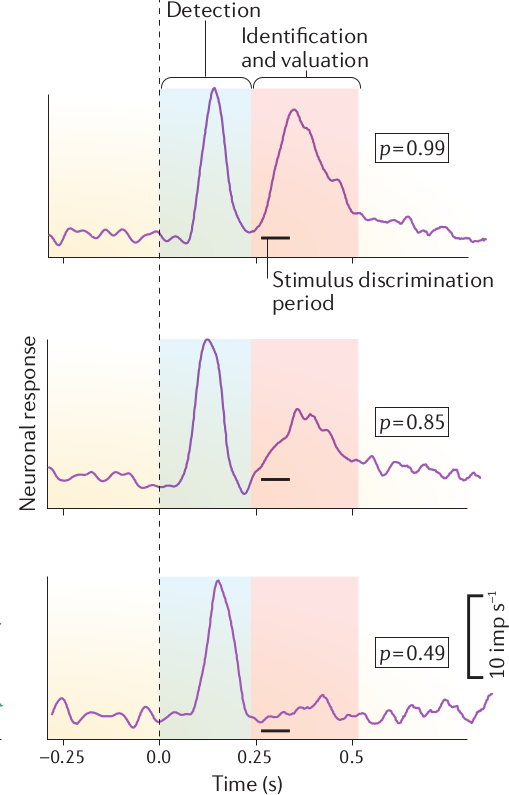
\includegraphics[scale=0.4]{figures/ResponseProbSchultz.png}
    \caption{Caption}
    \label{fig:probSchultz}
\end{figure}%These responses constitute biological implementation of the crucial error term for reinforcement learning. 
In this and further sessions an in-depth study of the task-related activity patterns of pair types is conducted, which will be linked to the coding features of the assembly-pairs.\\
We focused the analysis on those assemblies resulting significant for the Friedman test, the faction in percentage of those assemblies is shown in fig.\ref{fig:PercAsFried}. The histograms refer to the Friedman tests made on hit trials, in original and reversal phase separately.\\For each assembly-pair type we performed a large number of statistical tests, some will have p-values less than $0.05$ purely by chance, even if all null hypotheses of the family of tests performed are really true. Hence, to take this in account, Bonferroni correction for multiple comparison was applied. The Bonferroni correction is the classical approach to take in account the multiple comparison problem and consists in having a control on the familywise error rate ($\alpha=0.05$). This is possible by setting the critical value $\alpha$ for an individual test at lower value than 0.05, in such a way that if all the null hypotheses are true, the probability that the family of tests includes one or more false positives due to chance is 0.05. The value $\alpha$ for an individual test is obtained by dividing the familywise error rate by the number of tests.\\
\begin{figure}
    \centering
    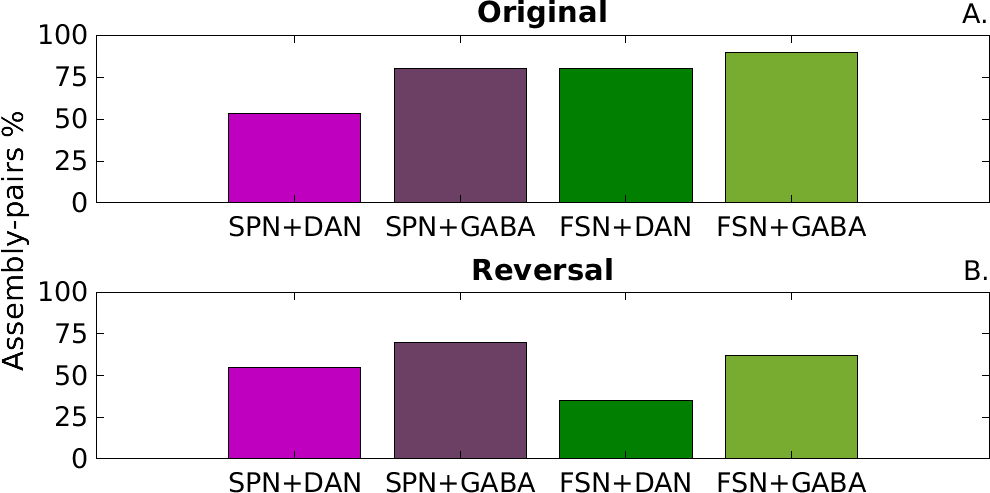
\includegraphics[scale=0.55]{figures/PercFriedHitTrialsBFf.png}
    \caption{Number in percentage of assembly-pairs exhibiting a significant task related pattern activity. The Bonferroni correction for multiple comparison was applied. In A. the significant assembly-pairs tested for the original phase, in B. the significant assembly-pairs tested in reversal. Assembly are divided in the four principal pair-types.}
    \label{fig:PercAsFried}
\end{figure}
Assembly-pairs patterns of significant assemblies were plotted, and differences in assembly-types emerged. In fig.\ref{fig:HeatPairsDan} assembly-pairs tested with Friedman test and resulting to have significant task related response in original phase. In order: A1. SPN-DAN assembly-pairs in original phase: a good portion of those pairs became active early at the rewarded stimulus (CS+) presentation, a good portion remains active during the stimulus presentation (CS+ cont.), until the reward retrieval (US), only a small fraction is active only in US window, this kind of answer makes those assembly-pair-types good candidate for reward prediction error coding. In A.2 the same assembly-pairs in the reversal phase. FSN-DAN assembly-pairs on contrast have a phasic response to the rewarded stimulus (CS+) and reward retrival (US) (B.1); in B.2 same FSN-DAN pairs in the reversal phase, a good portion of units responsive to CS+ in original phase, became in reversal responsive to US.\\ %This kind of answer makes those assembly-pair-types good candidate for Reward Prediction Error (RPE) coding.\\ 
Those consideration will be discuss in detail in \hyperref[sec:CorrRL]{Chapter~\ref*{sec:CorrRL}}, \hyperref[sec:Regression]{Chapter~\ref*{sec:Regression}}.\\From fig.\ref{fig:HeatPairsDan} and fig.\ref{fig:HeatPairsGaba} we have seen that different assembly-types are active in different task moments, summary plots are shown in fig. \ref{fig:FriedHistoDAN} and fig.\ref{fig:FriedHistoGABA} where we report in which windows (CS+, CS+ cont., US) assembly-pair are significantly active with respect to the baseline. The total amount can exceed the $100\%$ because if for example one pair was found significant in the US window and CS+ cont. with respect to the baseline, this assembly-pair was double counted.\\All assembly-pair types are predominantly active in the window $CS+ cont.$, that is the window of preparation for the reward.\\There differences among assembly-pairs types and phases. The first remarkable difference is between the original and reversal phase: in reversal phase for all pair-types we notice less activation in CS+ window with respect to the original phase. Assembly-pairs including SPN are in the reversal phase more active at retrieval (US). Assembly-pairs composed by GABA units became activated later than assembly-pairs composed by DAN.
 \begin{figure}
     \centering
     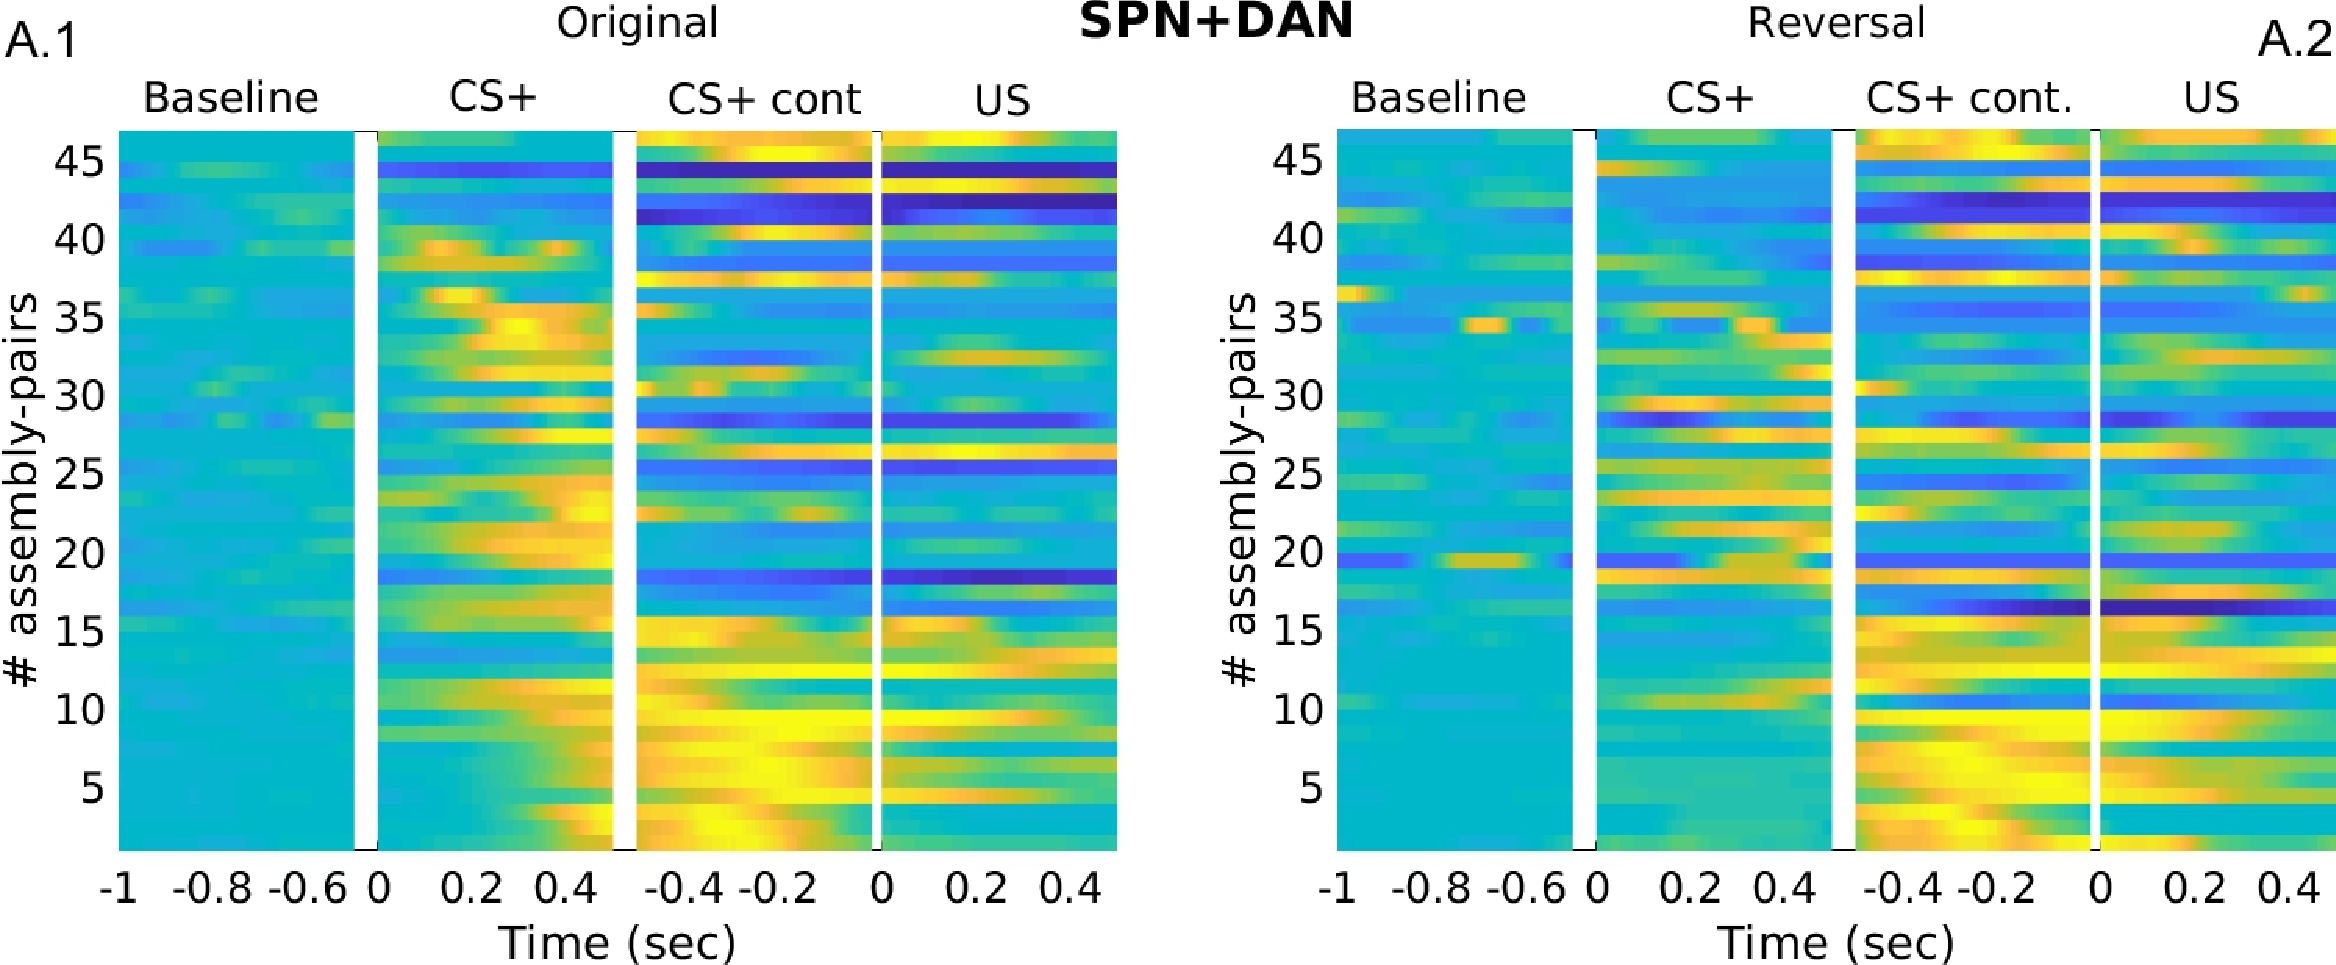
\includegraphics[scale=0.36]{figures/HeatSPN_DAN.pdf}
     
     \vspace{1cm}
     
     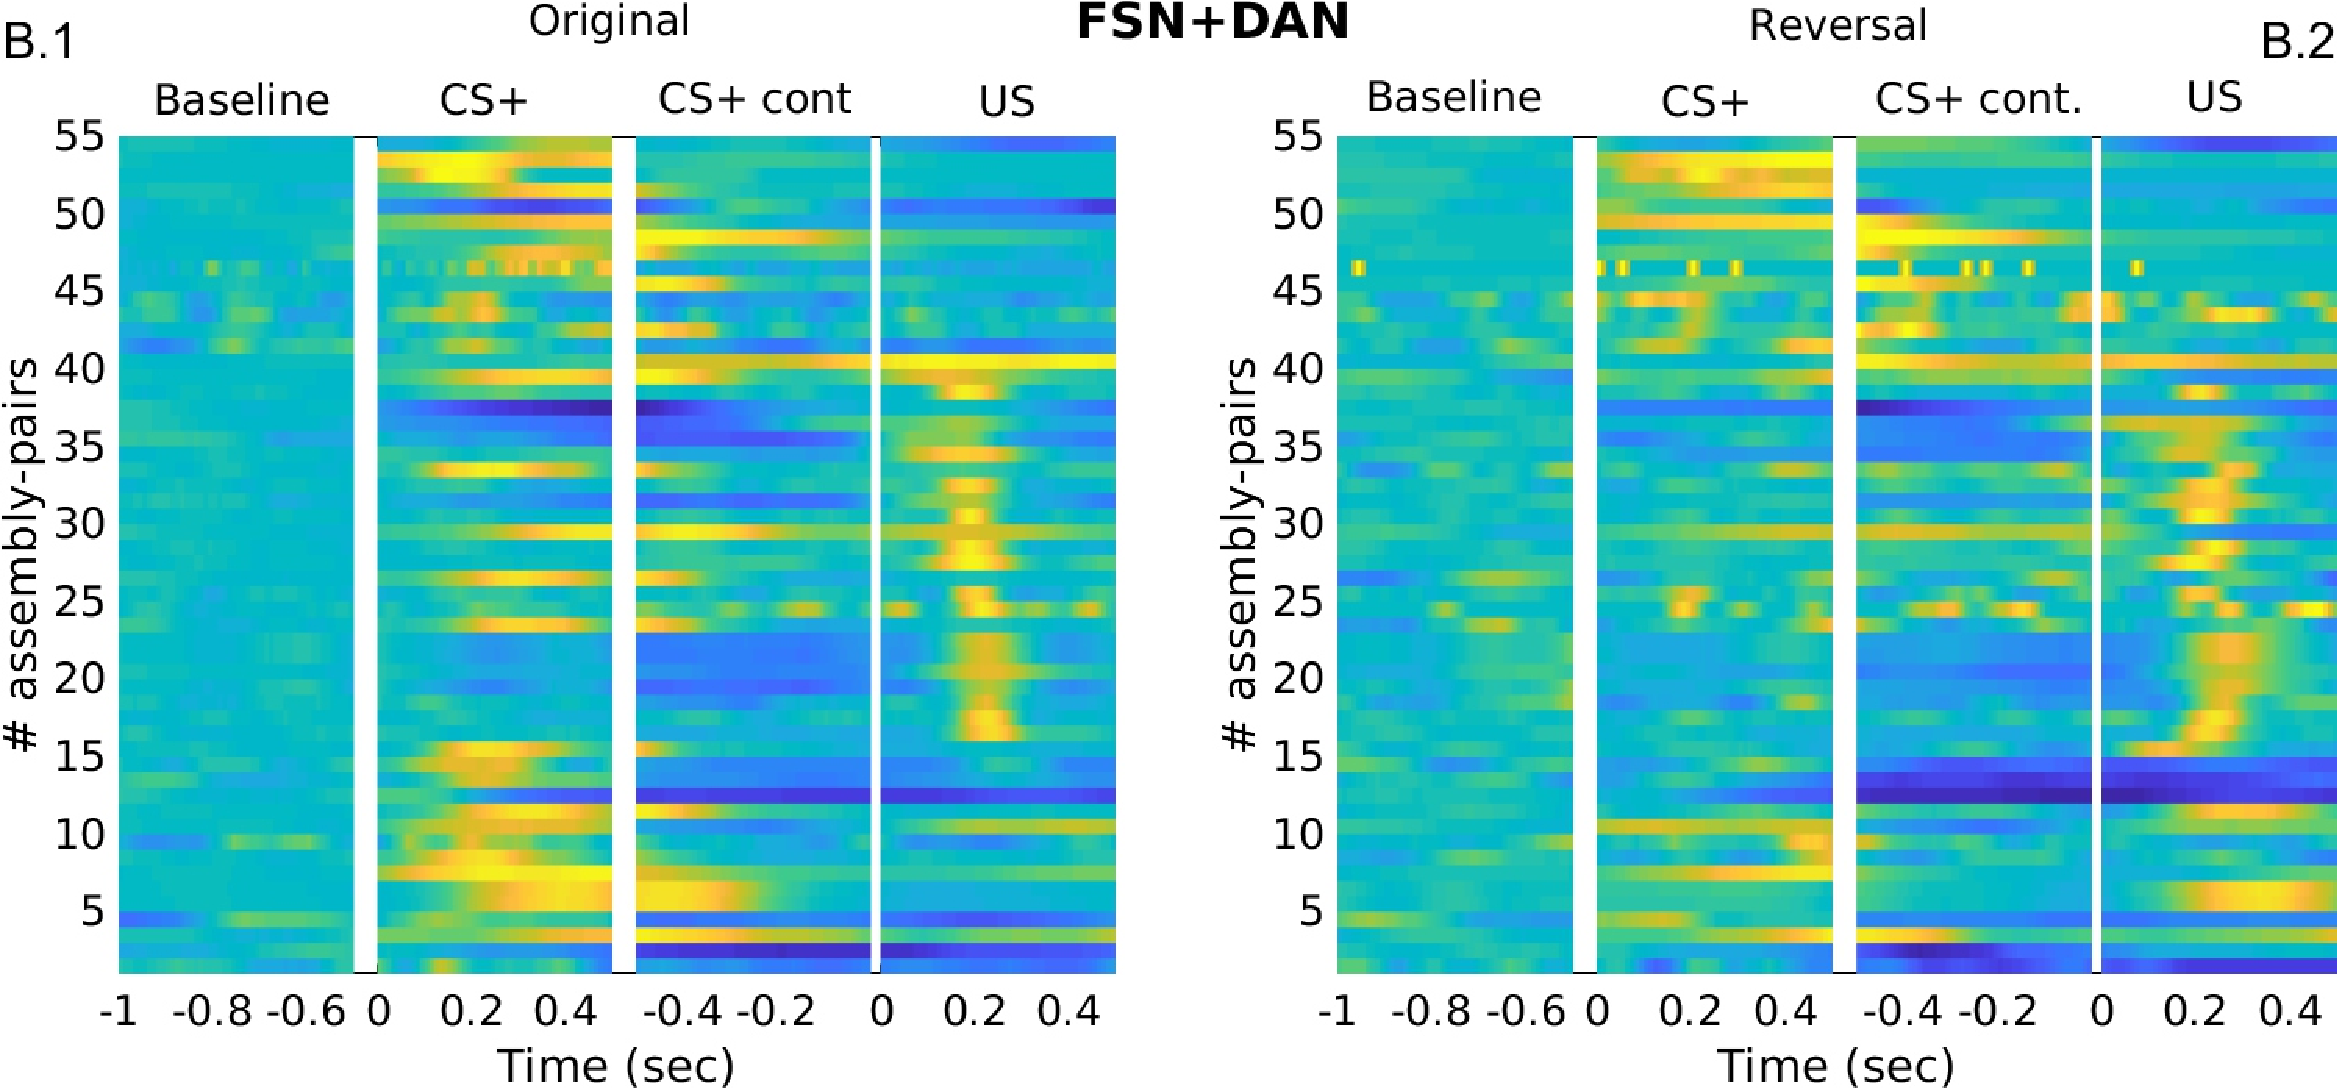
\includegraphics[scale=0.36]{figures/HeatFSN_DAN.pdf}
     \caption{Assembly-pairs tested with Friedman test and resulting to have significant task related response in original phase. In order: A1. SPN-DAN assembly-pairs in original phase: a good portion of those pairs became active early at the rewarded stimulus (CS+) presentation, a good portion remains active during the stimulus presentation (CS+ cont.), until the reward retrieval (US), only a small fraction is active only in US window, this kind of answer makes those assembly-pair-types good candidate for Reward Prediction (RP) coding. In A.2 the same assembly-pairs in the reversal phase. FSN-DAN assembly-pairs on contrast have a phasic response to the rewarded stimulus (CS+) and reward retrieval (US) (B.1); in B.2 same FSN-DAN pairs in the reversal phase, a good portion of units responsive to CS+ in original phase, became in reversal responsive to US. This kind of answer makes those assembly-pair-types good candidate for Reward Prediction Error (RPE) coding.}
     \label{fig:HeatPairsDan}
 \end{figure}
 \begin{figure}
     \centering
     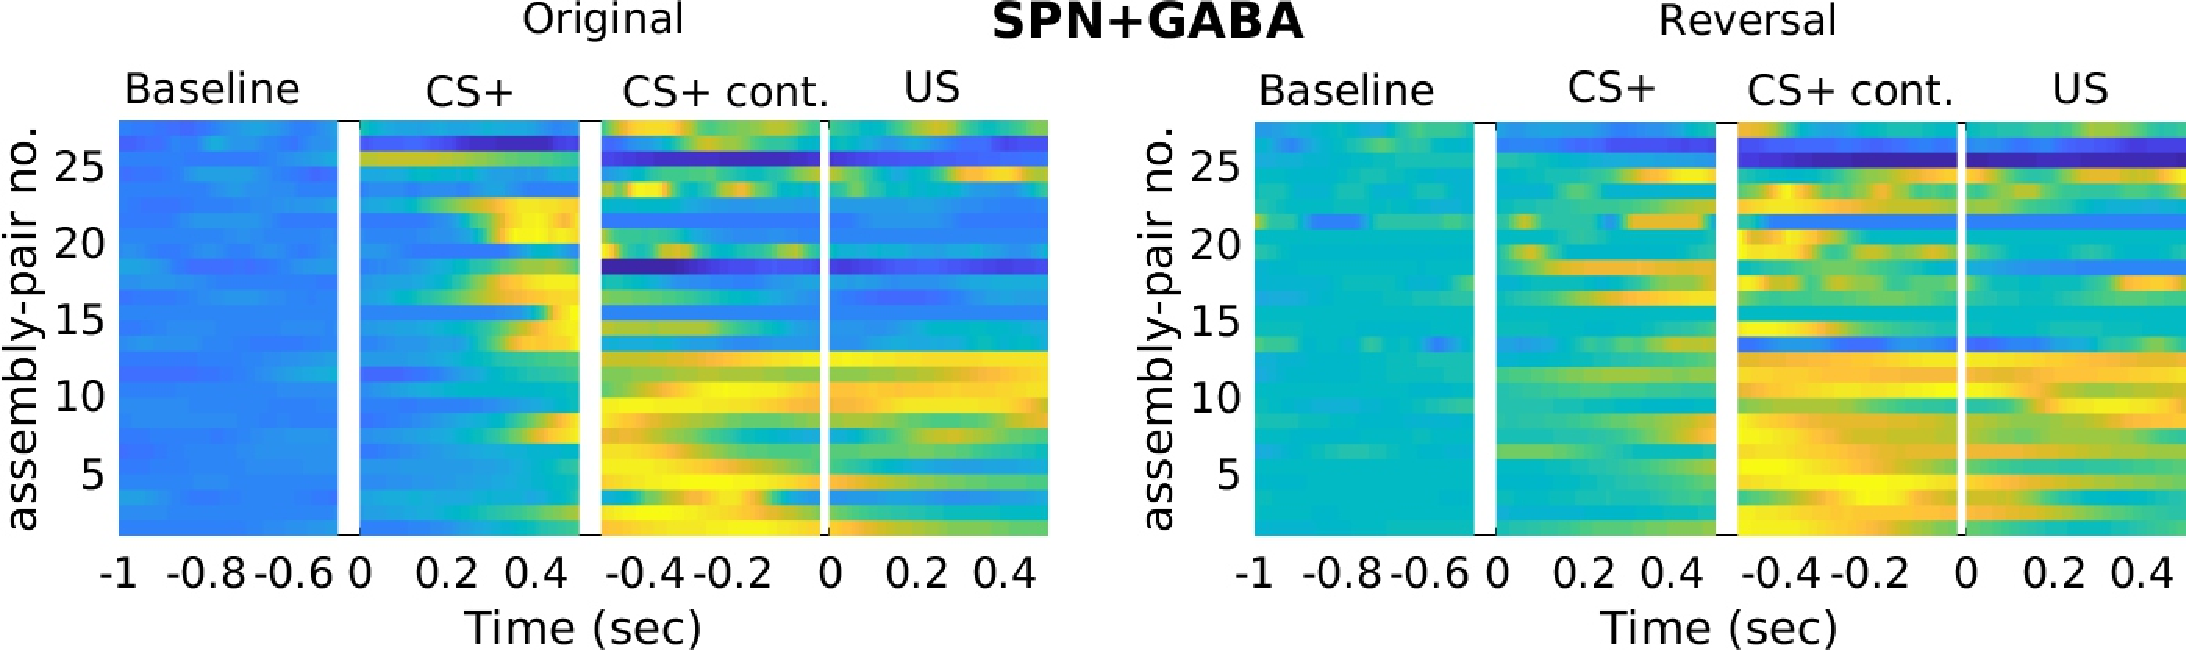
\includegraphics[scale=0.36]{figures/HeatSPN_GABA.pdf}
     
     \vspace{1cm}
     
     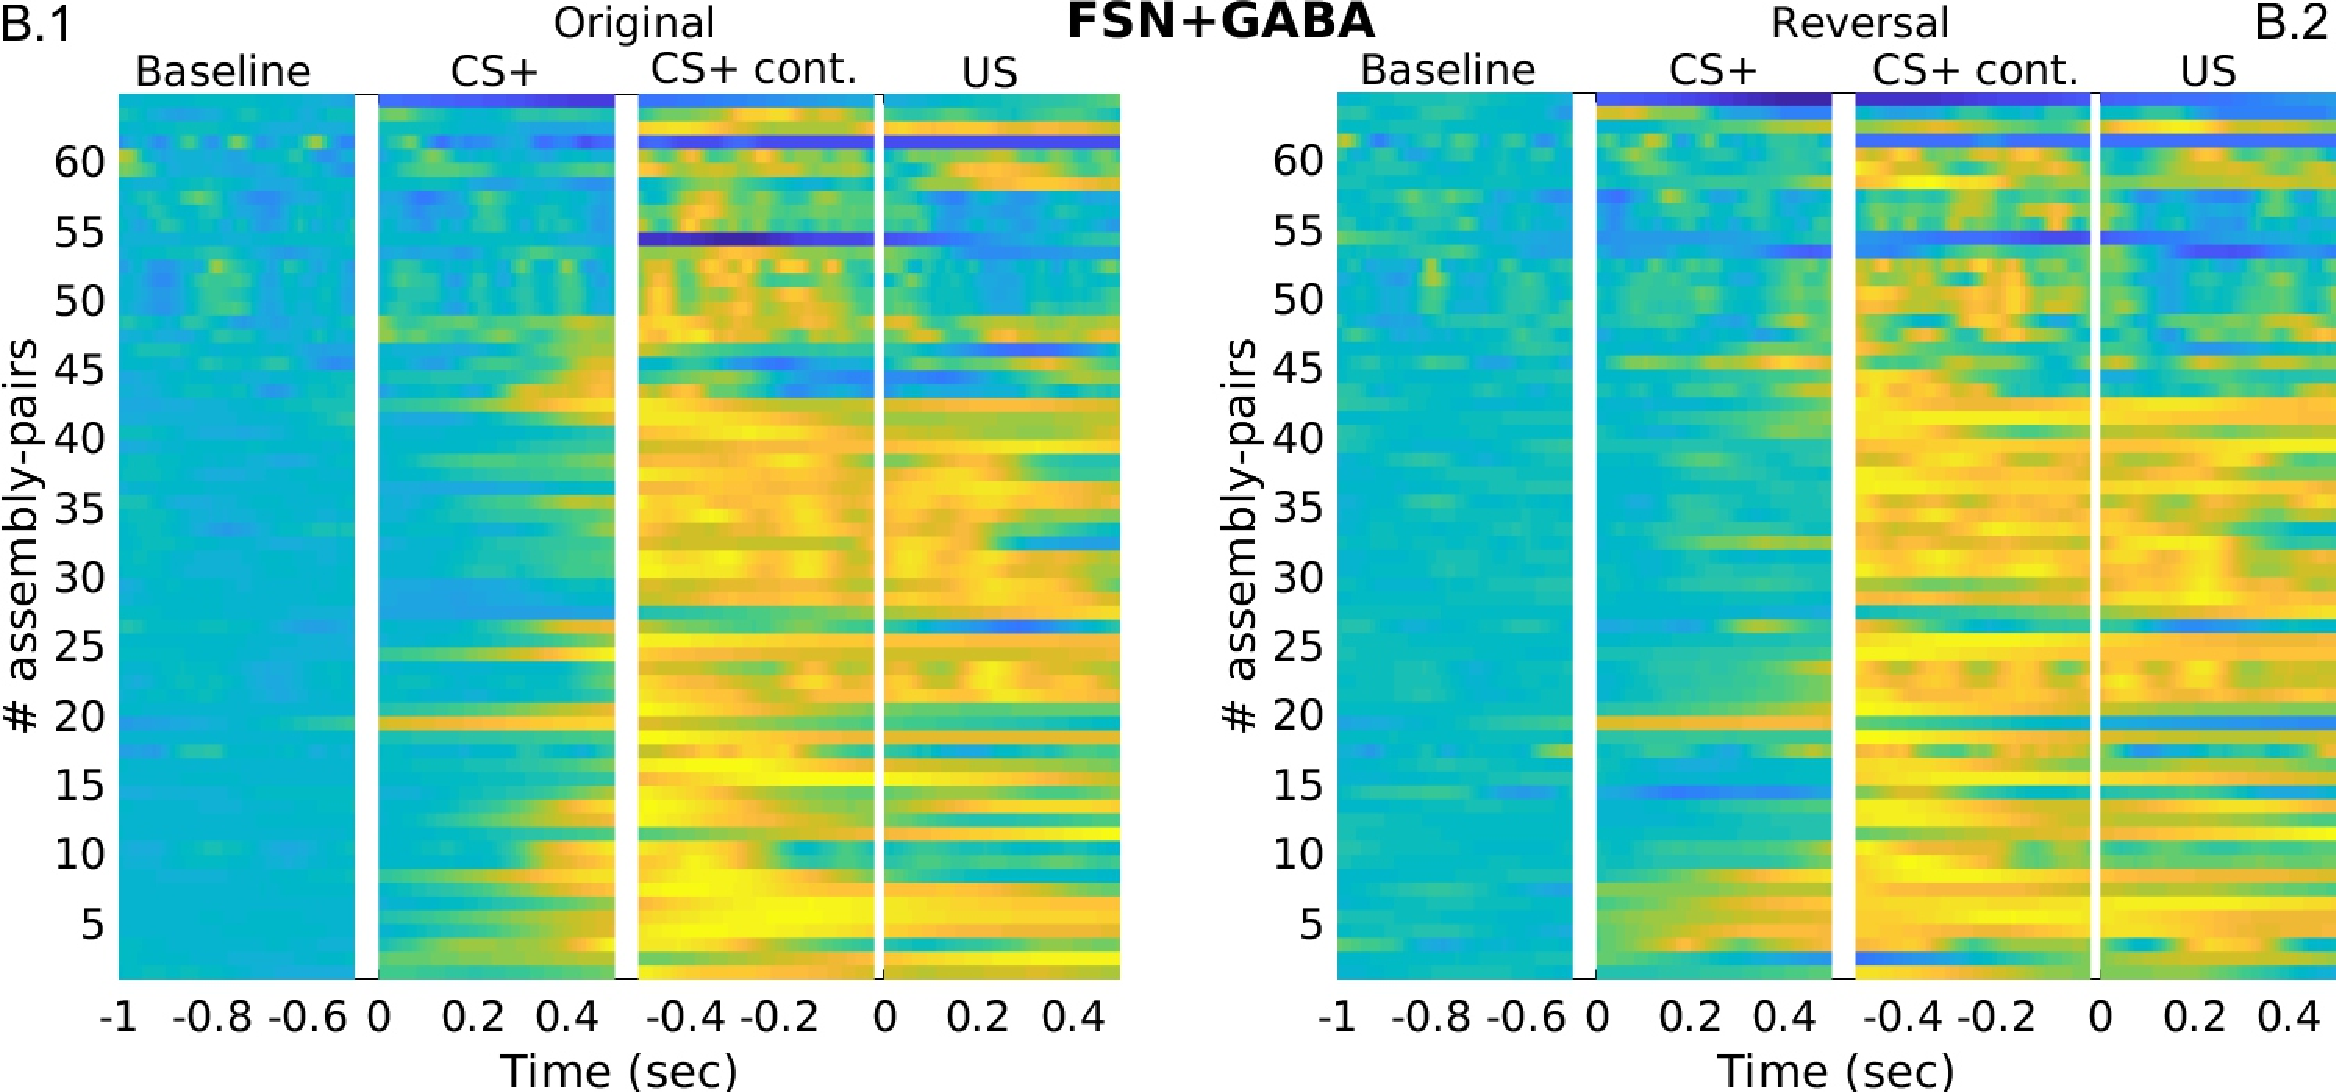
\includegraphics[scale=0.36]{figures/HeatFSN_GABA.pdf}
     \caption{Assembly-pairs tested with Friedman's test and resulting to have significant task related response in original phase. In order: in A.1 SPN-GABA assembly-pairs in original phase: a good portion of those pairs became active during the rewarded stimulus presentation (second half of CS+ and CS+ cont.), a good portion shows tonic activity until the reward retrieval (US). In A.2 the same assembly-pairs in the reversal phase. In B.1 FSN-GABA assembly-pairs are tonically active from the second half of the rewarded stimulus presentation window (CS+) to the reward retrieval window.}
     \label{fig:HeatPairsGaba}
 \end{figure}
 \begin{figure}
    \centering
    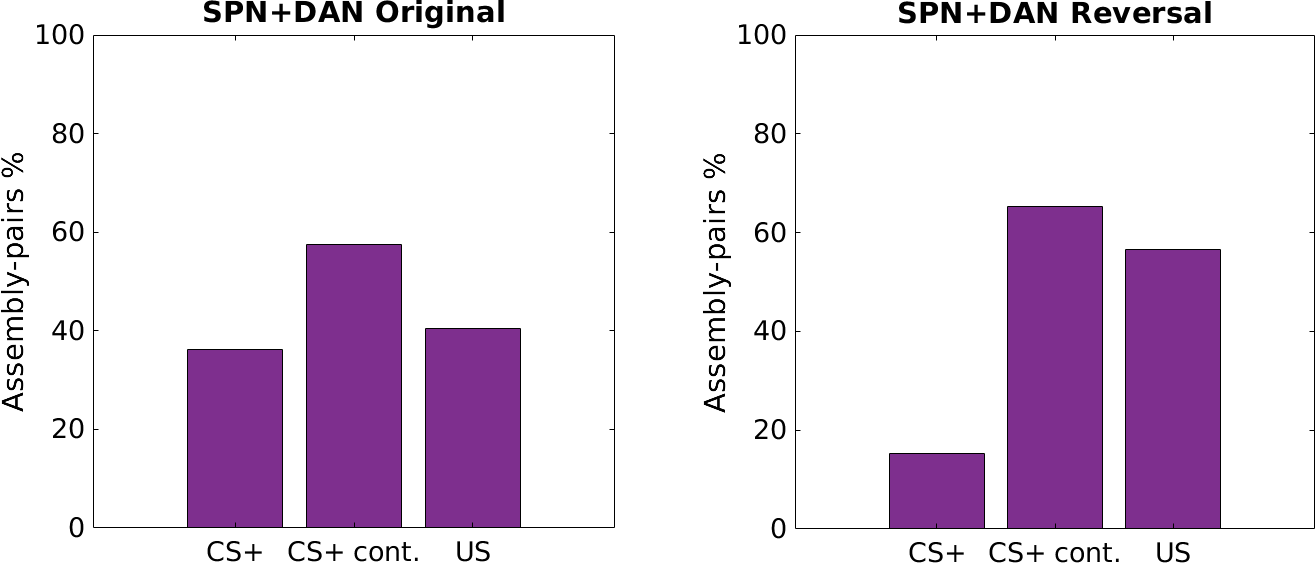
\includegraphics[scale=0.4]{figures/SPN_DANHisto.png}
    
    \vspace{1cm}
    
    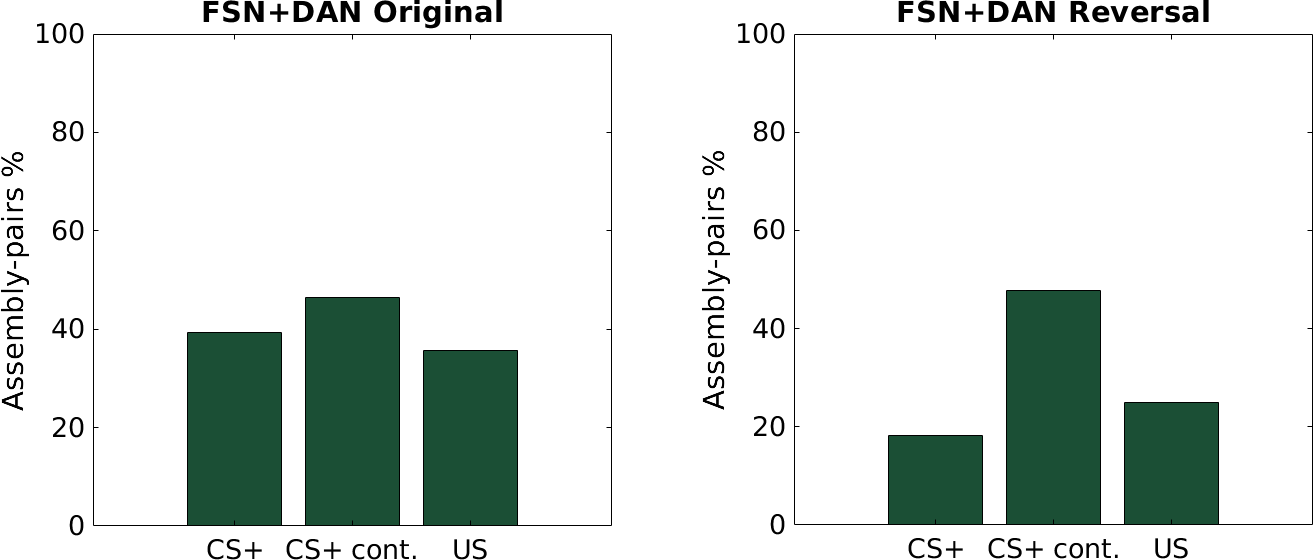
\includegraphics[scale=0.4]{figures/FSN_DANHisto.png}
\caption{Considering only the significant pairs we report the percentage of them significant with respect to the baseline in the windows $CS+$, $CS+ cont.$, $US$. The total amount can exceed the $100\%$ because if for example one pair were found significant in the US window and CS+ cont. with respect to the baseline, this assembly-pair was double counted.}
    \label{fig:FriedHistoDAN}
\end{figure}
\begin{figure}
    \centering
    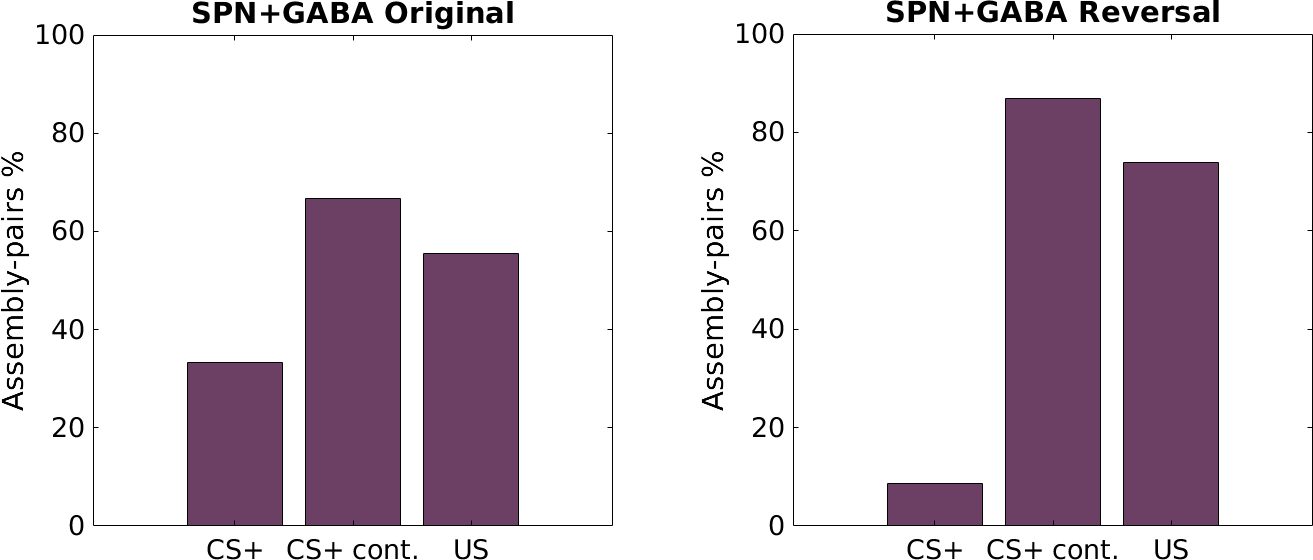
\includegraphics[scale=0.4]{figures/SPN_GABAHisto.png}
    
    \vspace{1cm}
    
    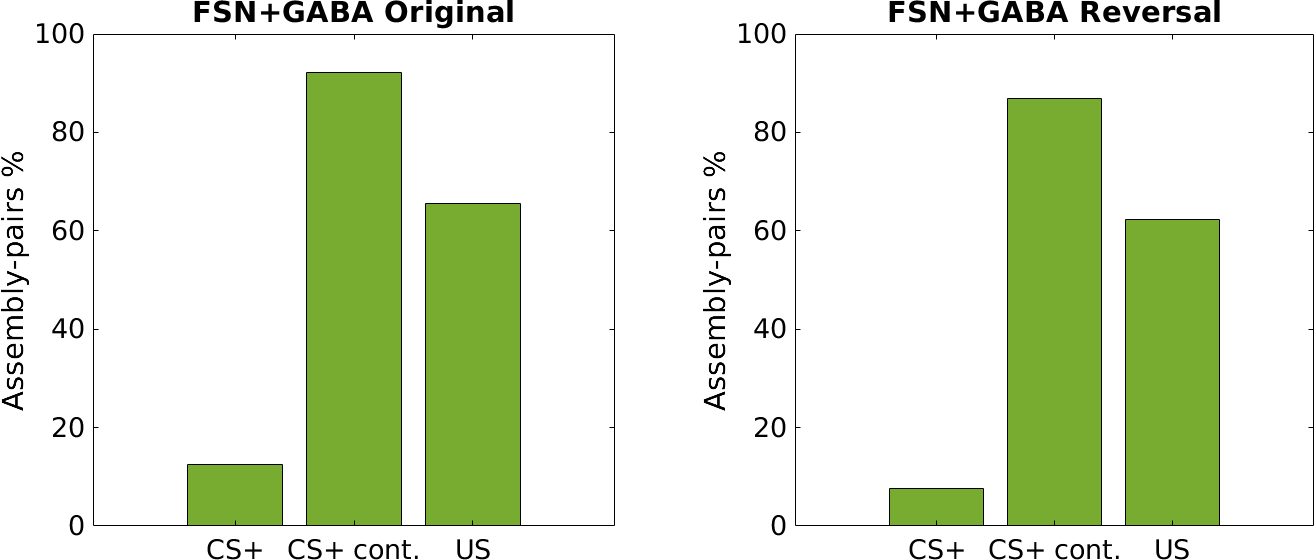
\includegraphics[scale=0.4]{figures/FSN_GABAHisto.png}
    \caption{Considering only the significant pairs we report the percentage of them significant with respect to the baseline in the windows $CS+$, $CS+ cont.$, $US$. The total amount can exceed the $100\%$ because if for example one pair were found significant in the US window and CS+ cont. with respect to the baseline, this assembly-pair was double counted.}
    \label{fig:FriedHistoGABA}
\end{figure}\\
\pagebreak
\section{False Alarm and Correct Rejection Trials}
{\color{red} discussion is a draft}
In the previous session we studied the assembly-pairs task related response in Hit trials, namely trials in which the odor was rewarded and the mouse went for the reward. We pruned assembly-pairs using a Friedman test to keep only assembly-pairs with significant task-related activation, in specific moment of the trial.\\In similar way we analyse the assembly-pairs task-related response for False Alarm trials (unrewarded odor, the mouse went for reward) and Correct Rejection trials (unrewarded odor, the mouse sat quiet).\\The three windows of interest were re-set up for these trials types in the following ways: in False Alarm trials those windows are called CS-, CS- cont., 3rd Lick. The CS- window, analogously to the CS+ in Hit trials, is a time interval of 0.5 $sec$ starting from the stimulus onset (unrewarded in this case); the CS- cont. and 3rd Lick are respectively the time intervals, again 0.5 $sec$ long, immediately before and after the expected reward.\\We used the following assumption to establish the expected reward time: since when the rewarded odor is presented the mouse has to lick at least two or three times depending on the paradigm to get the reward, when he goes for the reward even though the odor is unrewarded, he expects the reward after the second or the third lick depending on the paradigm used.\\In Correct Rejection trials the animal does not expect the reward, however we used as $"$hypothetical reward$"$ time, the average reward time obtained from Hit trials, to compare the assembly-pairs activity before and after the $"$hypothetical reward$"$ time with the activity before and after the reward time (Hit trials) or the expected reward time (False Alarm trials).\\The comparison between Hit, False Alarm and Correct Rejection is interesting because we expect different VS-VTA assembly-pair patterns in relation with reward prediction and reward occurrence, indeed dopamine is thought to be a key regulator of learning from appetitive as well as aversive events (\cite{Schultz1997}, \cite{Wenzel}, \cite{Fiorillo2013}, \cite{Schultz2015}).\\The predictive reward signal was widely studied in dopamine units (\cite{Schultz1998}, \cite{Schultz2001}, \cite{Doya}). When the animal receives reward unexpectedly, dopamine neurons fire a burst of action potentials. If a sensory stimulus reliably predicts reward, however, dopamine neurons decrease their response to reward, and instead burst to the stimulus, and finally if an expected reward is omitted, dopamine neurons pause their firing at the time they usually receive reward.\\
\begin{figure}
    \centering
    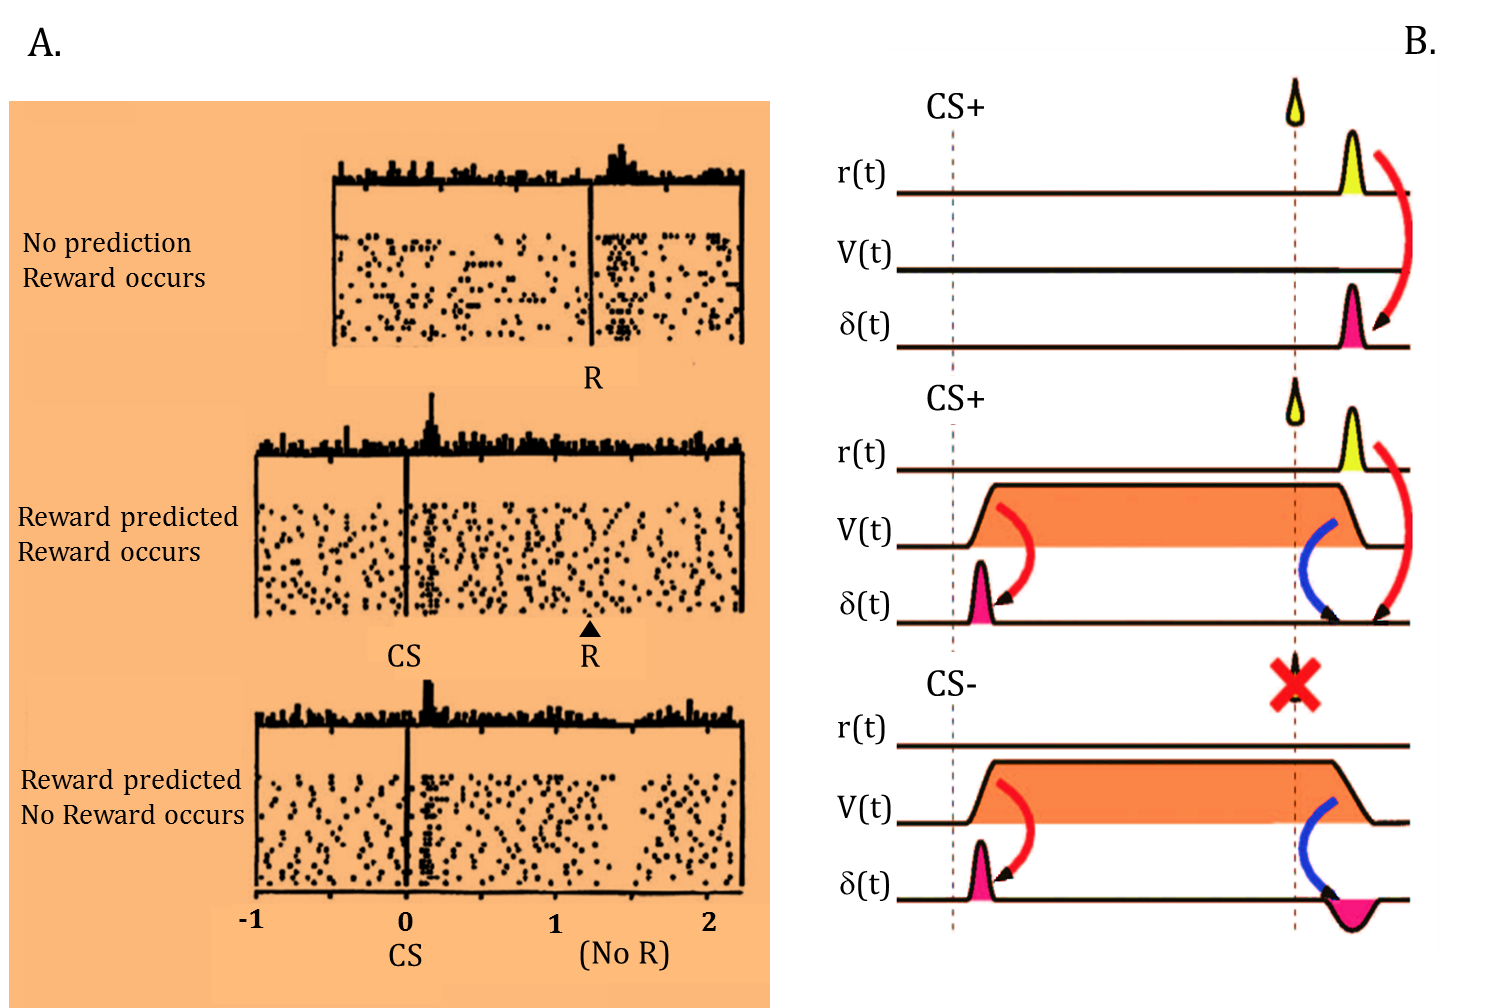
\includegraphics[scale=0.6]{figures/RewardDoyaRLSUM.png}
    \caption{Adapted from \cite{Doya}. In the first two panels response associated to rewarded trials. Last panel is related to unrewarded trials, in the cases in which the reward was predicted but it did not occur. Activity of the dopamine neuron is depressed exactly at the time when the reward would have occurred.}
    \label{fig:RewardDoya}
\end{figure}
In fig.\ref{fig:RewardDoya} (panel A.) is shown the predictive reward signal in dopamine units, whereas in panel B. we have a scheme of the learning where $r(t)$ stays for the reward, $V(t)$ is the expected reward, and $\delta(t)$ is the prediction error, namely the difference between the reward and the expected reward, that the animal computes at each trial when the reward is suppose to occur. From the top to the bottom, in both panels, the first two plots refer to rewarded trials, the third plot refers to unrewarded trials. The panel A. shows that in rewarded trials two kinds of activation are possible: an activation at the retrieval when the reward occurs but it was not predicted and activation right after the stimulus when the reward is predicted and it occurs, in this second case the activation at the retrieval disappears, whereas in unrewarded trials dopamine neurons are depressed. We assume that assembly-pair task related patterns reflect the predictive coding of underlying units, furthermore we expect that assembly analysis could reveal what is still discussed and unclear how predicted signal is formed in VS-VTA circuit.\\Recent works (\cite{UchidaDop}) shown that dopamine neurons exhibit homogeneity in response to both unexpected and expected rewards. Such uniformity ensures robust information coding, allowing each dopamine neuron to contribute fully to the prediction error signal. However remains untested whether a specialization in different aspects of prediction error is expressed through inter-regional patterns of coherence in the VS-VTA circuit. If the hypothesis of a specialized code is true, we would observe differences in activity patterns of VS-VTA assembly-pairs composed by dopamine units and different cell-types in VS.\\Interestingly we found that signals presented in the scheme \ref{fig:RewardDoya} are present both FSN-DAN pairs in hit trials (fig.\ref{fig:HeatFSN_DANComp}, panels A.1, A.2), and SPN-DAN pairs (fig.\ref{fig:HeatSPN_DANComp},panels A.1, A.2).\\Despite at first sight both assembly-pairs type seem to be involved in prediction coding, we want here emphasize the importance of the two components of the reward prediction-error signalling introduced in the previous session (\cite{Tobler2003}, \cite{Nomoto2010}, \cite{Fiorillo2013} \cite{Schultz2016}), and endorse the hypothesis that SPN-DAN pairs and FSN-DAN pairs are involved in different components of reward prediction coding.\\
In the previous session we introduced the two sequential components of neuronal response, called detection and identification/valuation, suggesting that sharp assembly-pairs FSN-DAN most probably code for generic identification of the stimulus, whereas SPN-DAN assembly pairs, characterized by broader response could code for the valuation, that is the component associated to the prediction error in reinforcement learning models.\\
\begin{figure}
    \centering
    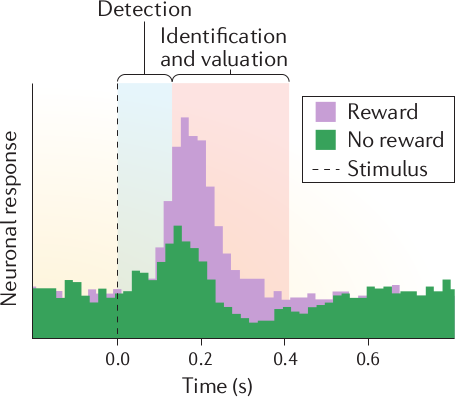
\includegraphics[scale=0.4]{figures/Schultz2016CSMod.png}
    \caption{Adapted from \cite{Schultz2016}. Voltammetric dopamine responses in rat nucleus accumbens distinguish between a reward-predicting conditioned stimulus (CS+) and a non-reward-predicting conditioned stimulus (CS-). The dopamine release comprises an initial indiscriminate detection component and a subsequent identification and value component.}
    \label{fig:dopCS}
\end{figure}
In fig.\ref{fig:dopCS} a useful comparison between neural responses in presence of rewarded and unrewarded stimulus. Again the comparison with the assembly-pairs suggests that SPN-DAN pairs code specifically for the valuation component.
SPN-DAN assembly-pairs show similar task-related patterns in Hit and and Correct Rejection trials (fig.\ref{fig:HeatSPN_DANComp}), interestingly in False Alarm trials we observed less stimulus activation with respect to the two correct realizations (Hit and Correct Rejection trials). This fact is guessed: the animal is indeed unsure about the stimulus received and performs wrong, while in correct trials, both Hit and Correct Rejection the animal is more confident\footnote{here a distinction between the early and the final stage of the task would be due, we leave this discussion to the next chapter.} about the output will be received, then, being able to predict the reward (or the absence of reward), reacts to the conditioned stimulus, that is again in agreement with the prediction error coding. As shown in fig.\ref{fig:dopCS} the mean response is anticipated in case of CS-, and again when CS- is presented often right after the identification a depression occurs. We assume SPN-DAN assembly-pairs being able to code for Reward Prediction and we prove this hypothesis in the next chapter.\\FSN-DAN assembly-pair activity patterns are more diversified among trials realizations, coherently with the hypothesis that they are unselective and multisensory in response. In Hit trials (fig.\ref{fig:HeatFSN_DANComp}, boxes A.1, A.2) the stimulus (CS+) leads an early activation, this activation can be associated with the initial component of the reward prediction error, namely the detection. In hit trials more than $\% 50$ of FSN-DAN pairs phasic activate at retrieval (US), suggesting that those pairs are not able to predict the reward. In False Alarm trials (fig.\ref{fig:HeatFSN_DANComp}, boxes B.1, B.2) the the stimulus presentation stimulus, unrewarded in this case (CS-), leads an activation of the majority of FSN-DAN pairs right after the stimulus presentation. In the windows before and after the expected reward (CS- cont., 3rd Lick) a good portion ($\sim50\%$) of FSN-DAN assembly-pairs show depression when the reward was predicted but it does not occur, probably coding for the frustration for realizing there will not be a reward, or some vague negative emotion. The assembly-pairs significant in original phase keep the same activation pattern in reversal with only slightly differences.\\One could observe that a similar inhibition was observed also in dopamine neurons when the reward was predicted and no reward occurred (see fig.\ref{fig:RewardDoya}, panel A, bottom), however in classical dopamine neurons activity the depression occurs in correspondence of the expected reward, while in FSN+DAN assembly-pairs the inhibition is anticipated in False Alarm trials, suggesting that they are involved in a different type of coding that is not (or only partially) represented by the classical reward prediction error definition used in reinforcement learning models.\\Finally we show FSN-DAN activity patterns in Correct Rejection trials (fig.\ref{fig:HeatFSN_DANComp}, boxes C.1, C.2): here we observe a good portion of FSN-DAN assembly-pairs is excitatory activated early by the stimulus presentation (CS- window), we observed also an inhibitory response in $\sim30\%$ of assembly-pairs, that can be interpreted as codification of the disappointment of the animal when the recognized unrewarded odor is presented, furthermore the $\sim10\%$ of assembly-pairs show an inhibitory response in CS- cont. window, after an excitation in CS- interval.
\begin{figure}
\centering
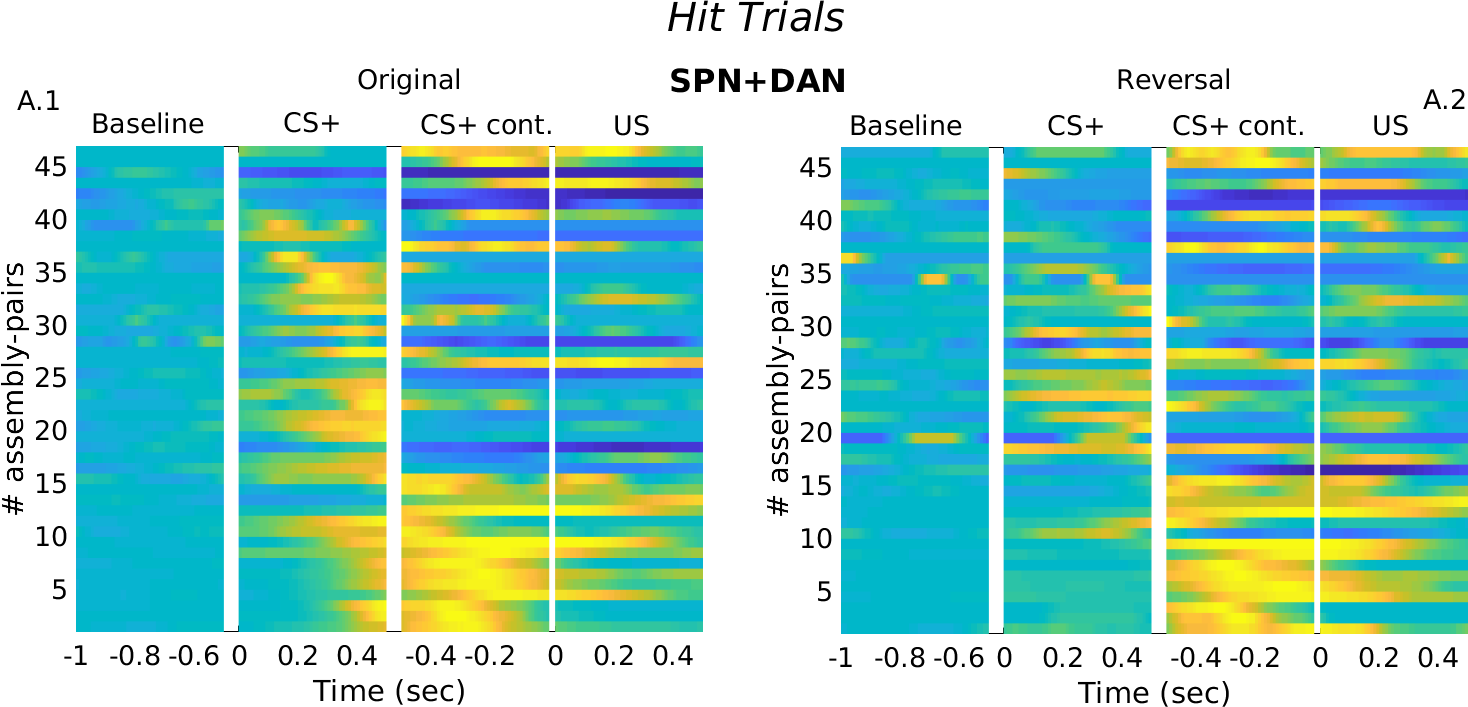
\includegraphics[scale=0.36]{figures/HeatSPN_DANHit.png}
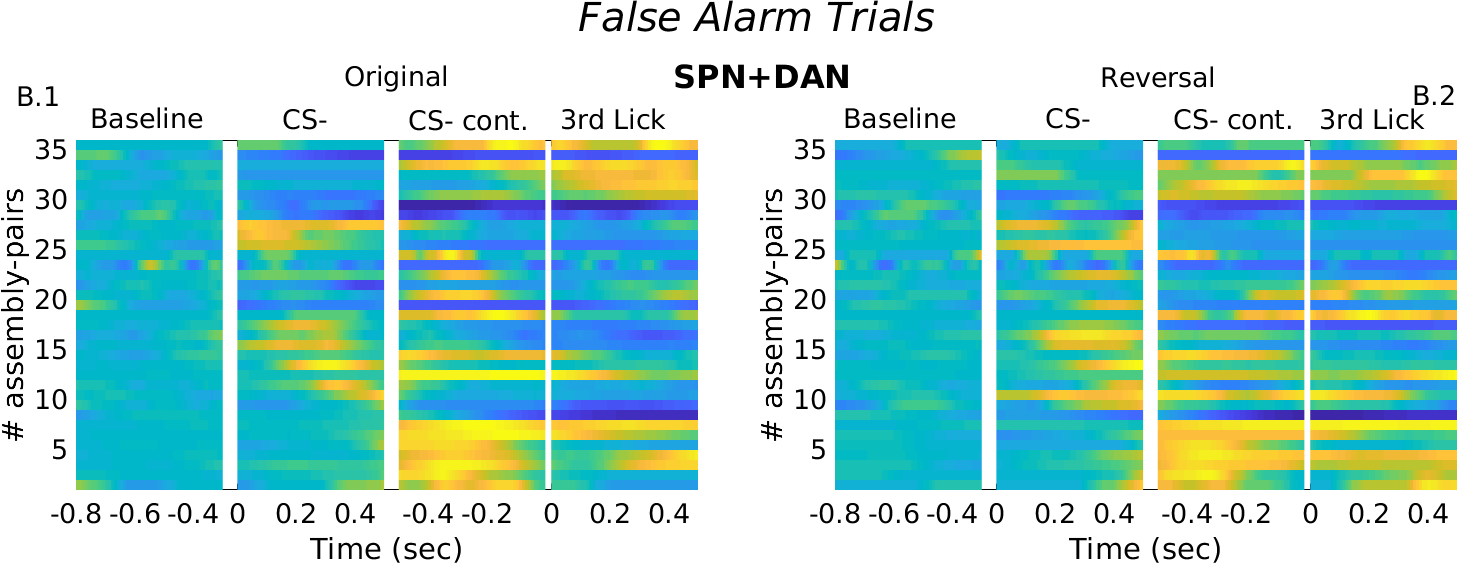
\includegraphics[scale=0.36]{figures/HeatFA_SPN_DAN1.png}
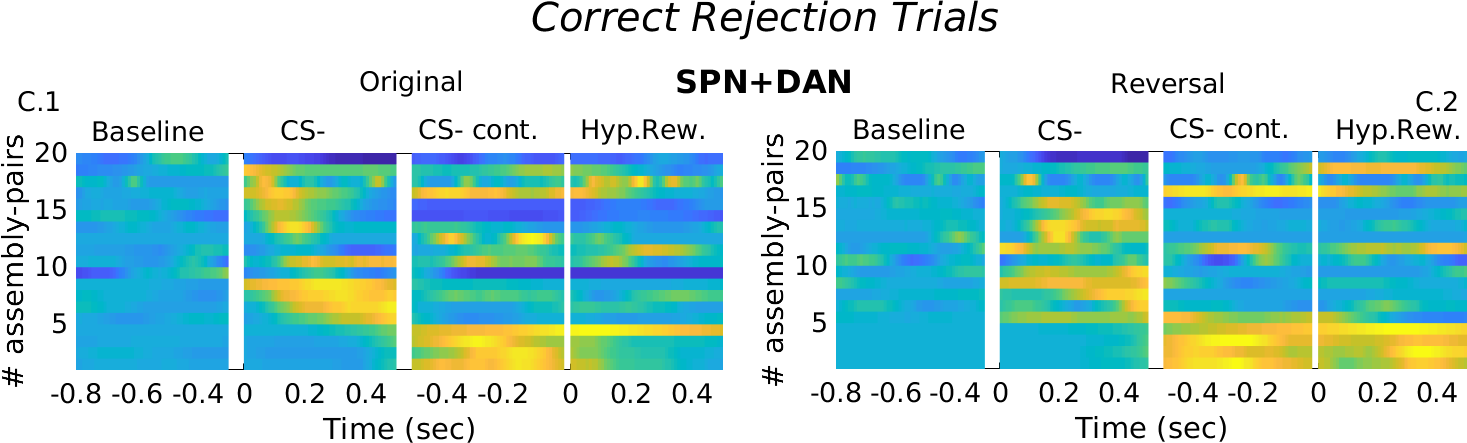
\includegraphics[scale=0.36]{figures/HeatCR_SPN_DAN1.png}
\caption{SPN-DAN assembly-pairs significant for Friedman test in three trial realizations (Hit, False Alarm and Correct Rejection). SPN-DAN pairs show similar pattern of activity in the three realizations, however it is worth to remark in False Alarm trials less activation at the stimulus presentation and a group of pairs at the expected reward time. In Correct Rejection trials $\sim 80\%$ of pairs are early activated by the stimulus (CS-).}
\label{fig:HeatSPN_DANComp}
\end{figure}
 \begin{largefigure}[20pt]
 \centering
 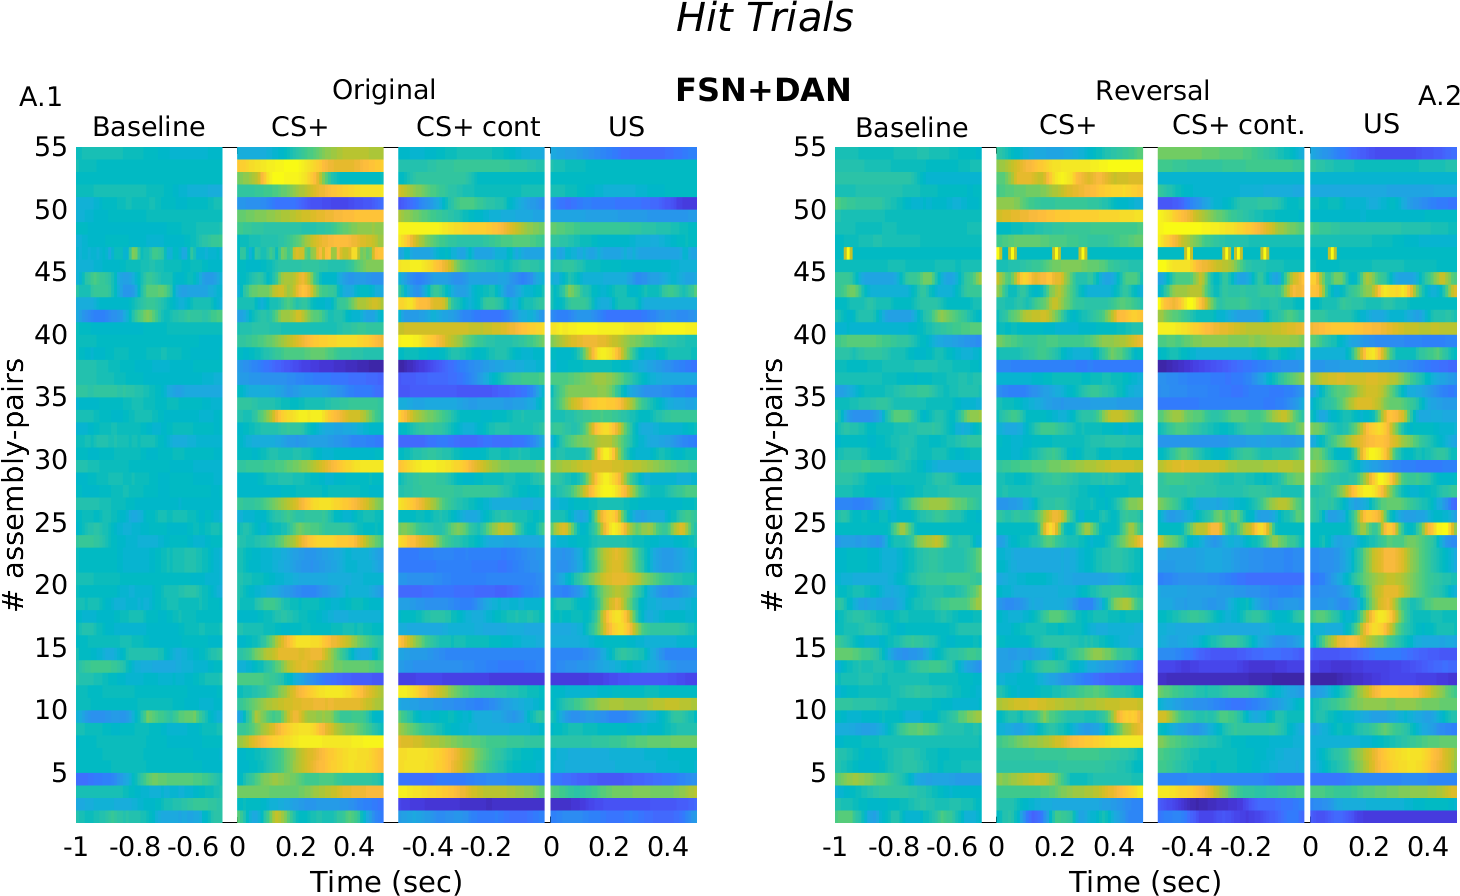
\includegraphics[scale=0.3]{figures/HeatFSN_DANHit.png} 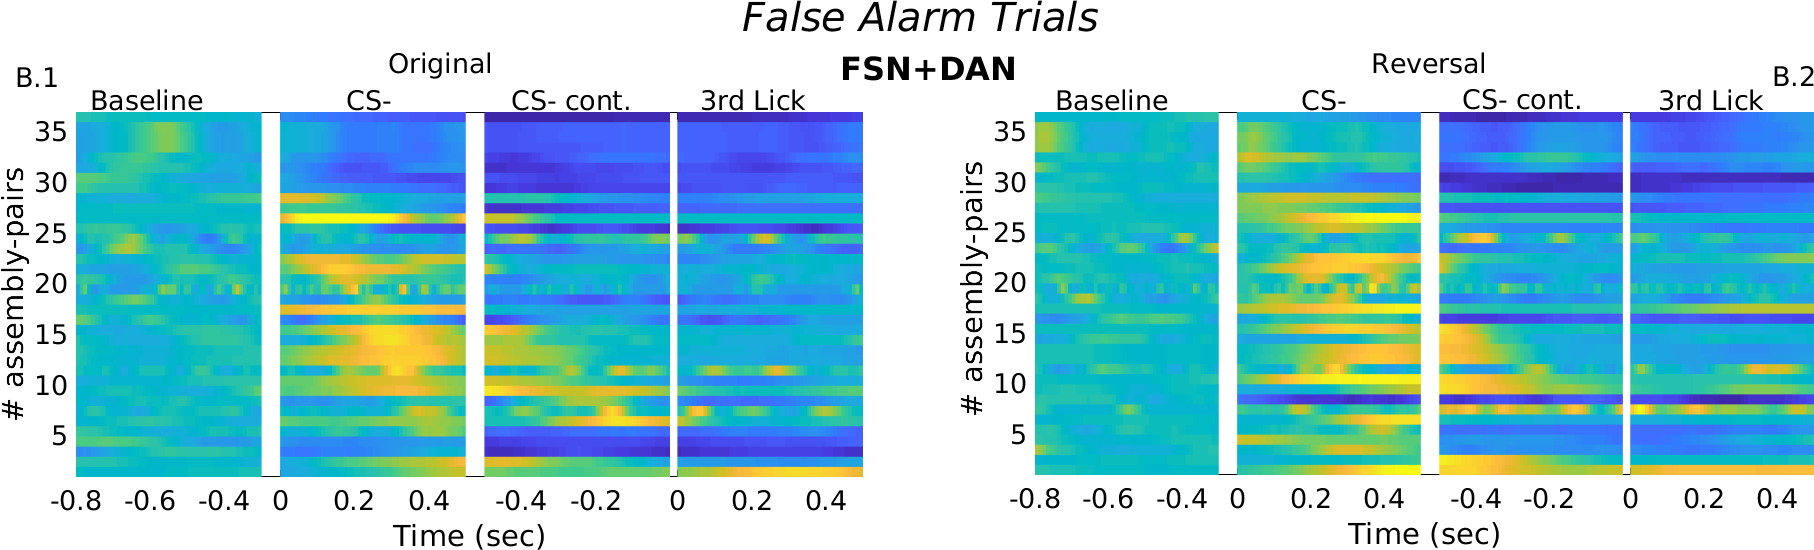
\includegraphics[scale=0.3]{figures/HeatFA_FSN_DAN1.png}
 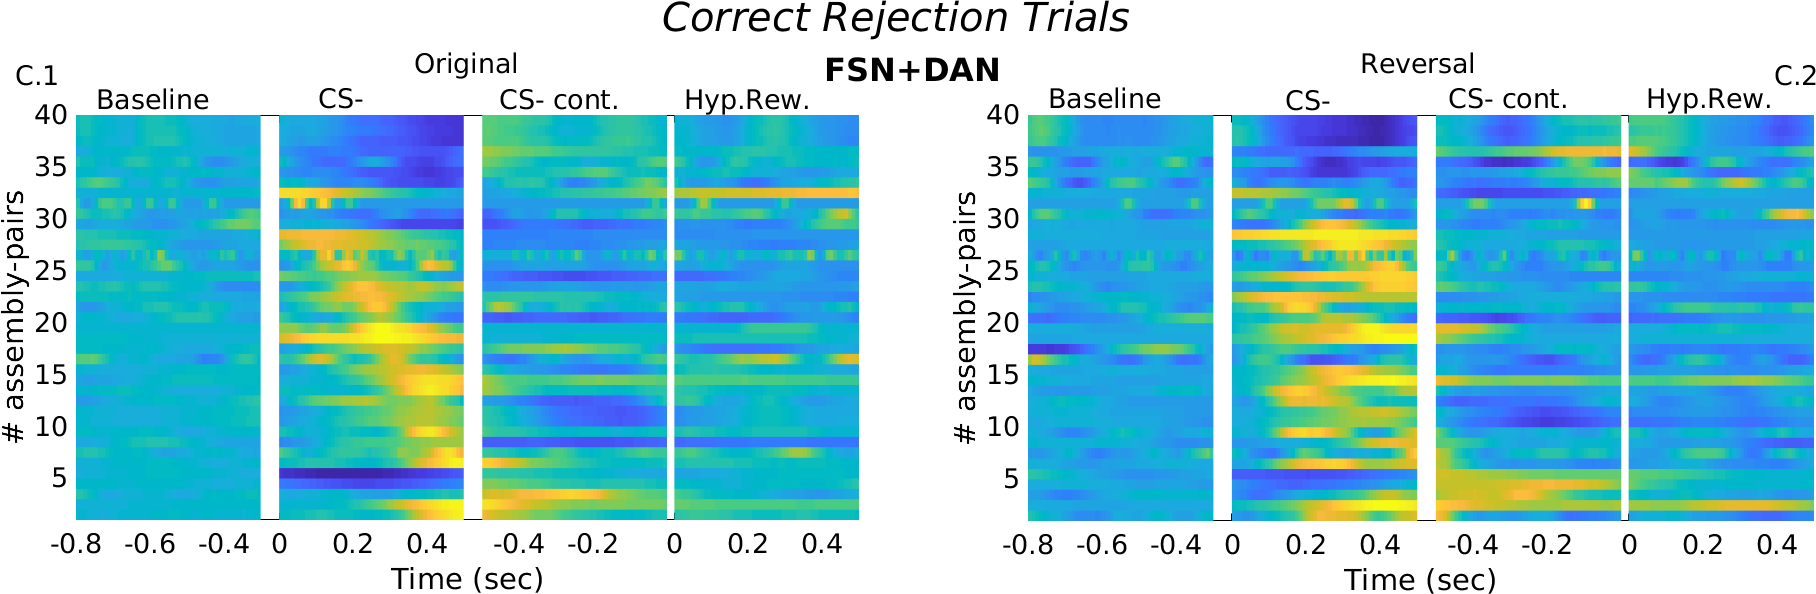
\includegraphics[scale=0.3]{figures/HeatCR_FSN_DAN1.png}
  \caption{FSN-DAN assembly-pair activity patterns are diversified among trials realizations. In Hit trials (A.1, A.2) early stimulus (CS+) response and a phasic response on retrieval (US), in False Alarm trials (boxes B.1, B.2) the activation to the stimulus remains, no excitatory activation in the windows before and after the expected reward time. Instead we observe a good portion ($\sim50\%$) of FSN-DAN assembly-pairs showing inhibitory activity with respect to the baseline. In Correct Rejection trials (boxes C.1, C.2) a good portion of FSN-DAN assembly-pairs is excitatory activated early by the stimulus presentation (CS- window), $\sim30\%$ of assembly-pairs exhibits inhibitory response, the $\sim10\%$ of assembly-pairs shows an inhibitory response in CS- cont. window, after an excitation in CS- interval.}
  \label{fig:HeatFSN_DANComp}
\end{largefigure}
\pagebreak

\section{Conclusion}
{\color{red} this part is a draft. Rephrase properly hypothesis!!!! clear hypothesis on SPN-DAN and FSN-DAN need to emphasized }
In the previous two sections we extensively described the task-related activity of assembly-pair types. We first noticed that different assembly-pairs types show different task-related patterns of activity, and consequently they could exhibit different coding feature.\\The observed activity patterns, at the stimulus presentation and at the retrieval, let to suppose that VS-VTA pairs are able to integrate the difference between expected and received outcomes.\\ Typical single neuron activity in VS and VTA related to expectancy of reward and uncertainty was largely investigated in last decades (\cite{Fiorillo}, \cite{Schultz}, \cite{Schultz1992}, \cite{Schultz1998}), however how the VS-VTA interaction could form and encode those kind of signals is not fully understood. As first step we made a parallelism between the single unit activity related to probability of reward and the activity exhibited by the detected assembly-pairs.\\From the resemblance of their response we have been able to assume that SPN-DAN assembly-pairs could code for reward prediction (RP).\\Despite FSN-DAN pairs seem to not code for the second component of prediction error, given the persistent activation at the retrieval, they show 
interesting behavior in False Alarm trials, where $\sim 50\%$ of FSN-DAN pairs show inhibitory responses before the rewarded was expected, from which one can guess the $"$disillusionment$"$ coding, whereas in Correct Rejection trials $\sim 30\%$ of FSN-DAN pairs shows an inhibitory response already at the presentation of the recognized rewarded odor, from which one can guess an ability of those pairs to code for the $"$disappointment$"$ related to the consciousness of not getting the reward.\\However FSN-DAN pairs seems to be involved in reward prediction error computation in a different way that SPN-DAN pairs, they unspecifically react to the stimulus in response. The unselective and multisensory nature of their response could correspond to a very braod range of coding futures that is only partially explained by the reward prediction error definition.\\From SPN-DAN pair activity patterns and FSN-DAN activity patterns, it emerges a clear specificity of assembly-pairs, suggesting that different assembly-pairs specialize in different aspects of prediction error, whereas was tested that at single units level responses of dopamine neurons to both expected and unexpected rewards follows the same function (\cite{UchidaDop}).\\Next chapter is entirely dedicated to prove the hypothesis of specificity of inter-regional pairs in reward related signal. In particular we asked whether SPN-DAN or FSN-DAN pairs are involved in prediction coding during a learning process, and if they share common response function for reward prediction error.\\The analysis shown until this point is static and cannot fully answer this question. The prediction signal is considered to be the basis of associative learning (\cite{RescorlaWagner}), and bears a striking resemblance to machine learning algorithms (\cite{SuttonBarto}). Thus, to address the aforementioned question we pass to a dynamic vision introducing the learning dynamic through a machine learning model.

 %%%%%%%% Commento forse da buttare
 %First difference between original and reversal phase is number of assemblies responding during the post-stimulus interval, this number decrease for all the typologies involved during hit trials (as shown in fig. (\ref{fig:histo_taskrel})), in according to the intuition, in reversal phase in fact, when the animals became more expert, neuronal response tend to be shifted closer to the reward delivery. This effect can be seen in fig. (\ref{fig:NeusInAsse}) where activity and raster plots of two units in a pair are shown. Looking at the raster plots, a shift in correspondence to the phase-switch is evident in both units.
 %\begin{figure}
  %   \centering
  %   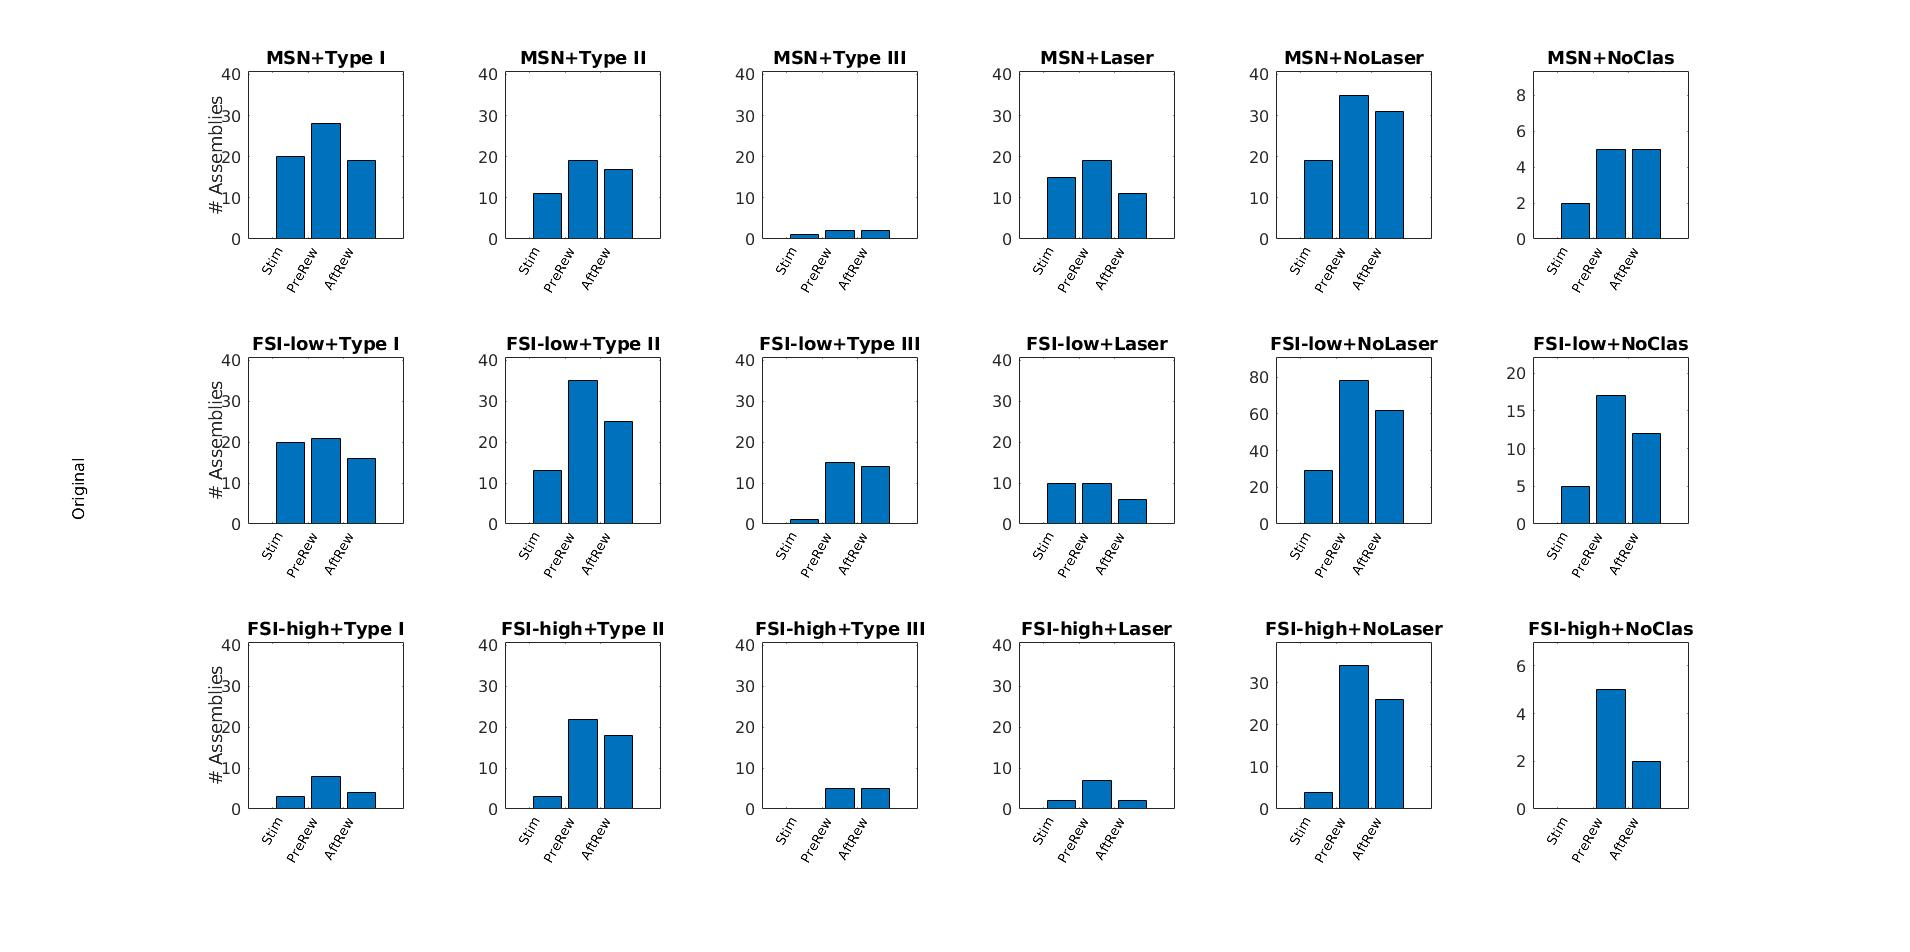
\includegraphics[scale=0.3]{figures/Original_Hit_N.jpg}
    % 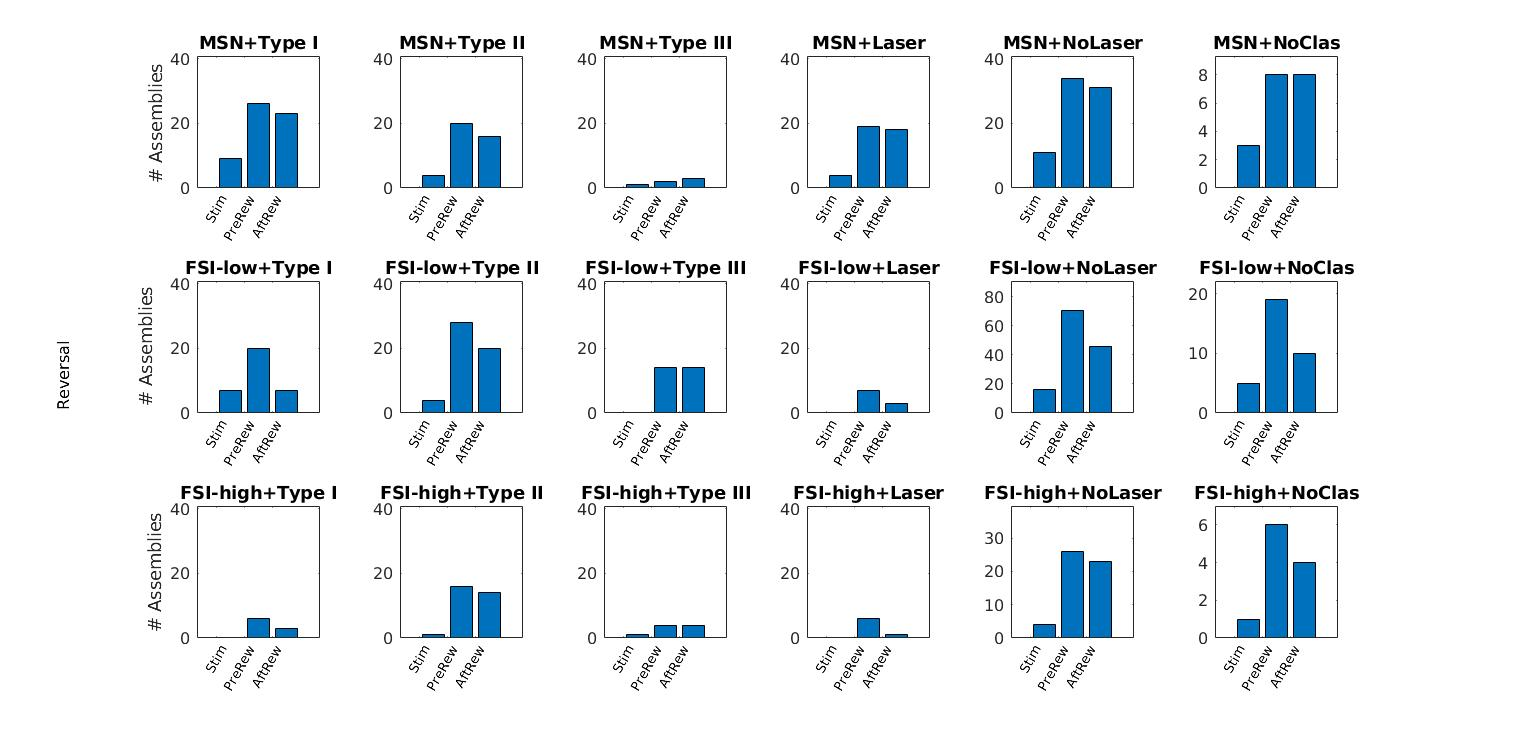
\includegraphics[scale=0.3]{figures/Reversal_Hit_N.jpg}
     %\caption{{\color{red}TO MODIFY!!!! BUT THIS IS THE PLOT}}
     %\label{fig:histo_taskrel}
 %\end{figure}
%\begin{figure}
  %  \centering
   % 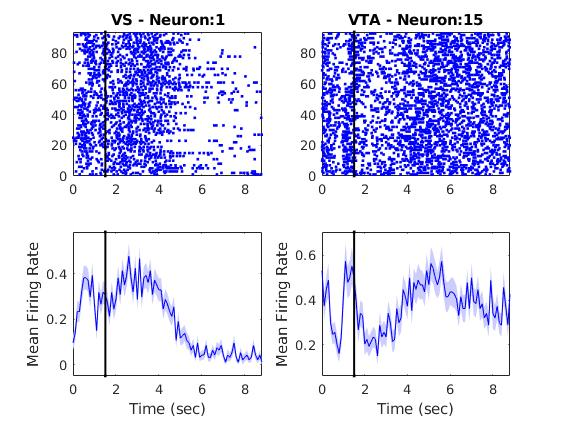
\includegraphics[scale=0.6]{figures/SingleNeus1_15Lastrev1Pru_An_4.jpg}
    %\caption{Shift in time of neuronal activity of two units in assembly. }
    %\label{fig:NeusInAsse}
%\end{figure}

%\section{Discussion}
%\section{Combination of single neuron and assemblies analysis}
%\subsection{Directionality using classification}
%\subsection{Significant task related response for typology}
%%%%%%% Fine Commento forse da buttare


%%%%% Commento Utile
%To better study assemblies activation patterns, first the task relevant moments of the experiment were selected. From the mean task related activity patterns we expected to see differences among assemblies types in two experimental chapters (original and reversal). To better visualize the task related activation patterns via heat plots, hit trials (rewarded odor, mouse went for reward), correct rejection trials (unrewarded odor, mouse sat quiet), false alarm trials (unrewarded odor, mouse went for reward), were kept separated; however this separation among trials types was released in further analysis, without affecting results.
%The assemblies were pruned according their significant task related activity, that was tested with Friedman's test and a non parametric version of the repeated measures Anova. We preferred to use non-parametric tests to be free from the assumption of gaussianity of the observations. Results of the two tests were consistent each other. The two relevant events of the task were the odor onset and the reward delivery, then we choose whether the assemblies showed a significant activity in three windows: Stimulus [0s, 0.5s], Pre-Reward [-0.5s, 0s], Reward [0s, 05s], the baseline was chosen in the interval [-1s, -0.5s] from the odor onset. Post-hoc analysis were performed using the Bonferroni's criterion {\color{red}check whether the criterion was Bonferroni of some other}. Almost $80\%$ of the VS-VTA assemblies showed a task related activity significant different from the baseline or from another of the windows considered. Of the significant assemblies $\%$ were composed by MSN-Type I units, $\%$ by FSI low-Type I, $\%$ by FSI high-Type I, $\%$ MSN-Type II, $\%$ by FSI low-Type II, $\%$ by FSI high-Type II, the other possible units combinations constitutes a minority and all toghether were the $\%$ {\color{red} Insert numbers of percentage}.

%\section{Conclusion}
